% 导入配置
% \documentclass[lang = cn, scheme = chinese, thmcnt = section]{elegantbook}
% elegantbook      设置elegantbook文档类
% lang = cn        设置中文环境
% scheme = chinese 设置标题为中文
% thmcnt = section 设置计数器


%% 1.封面设置

\title{Algebra Chapter 0 - Paolo Aluffi - NoteBook}                % 文档标题

\author{若水}               % 作者

\myemail{ethanmxzhou@163.com} % 邮箱

\homepage{helloethanzhou.github.io} % 主页

\date{\today}               % 日期

\extrainfo{上善若水任方圆}   % 箴言

\logo{PiCreatures_happy.pdf}        % 设置Logo

\cover{阿基米德螺旋曲线.pdf}          % 设置封面图片

% 修改标题页的色带
\definecolor{customcolor}{RGB}{135, 206, 250} 
% 定义一个名为customcolor的颜色,RGB颜色值为(135, 206, 250)

\colorlet{coverlinecolor}{customcolor}     % 将coverlinecolor颜色设置为customcolor颜色

%% 2.目录设置
\setcounter{tocdepth}{3}  % 目录深度为3

%% 3.引入宏包
\usepackage[all]{xy}
\usepackage{bbm, svg, graphicx, float, extpfeil, amsmath, amssymb, mathrsfs, mathalpha, boondox-cal, boondox-calo, hyperref, graphicx, romannum, chemarrow, booktabs, fontspec, ctex}

%% 4.定义命令
\newcommand{\N}{\mathbb{N}}            % 自然数集合
\newcommand{\R}{\mathbb{R}}            % 实数集合
\newcommand{\C}{\mathbb{C}}  		   % 复数集合
\newcommand{\Q}{\mathbb{Q}}            % 有理数集合
\newcommand{\Z}{\mathbb{Z}}            % 整数集合
\newcommand{\F}{\mathbb{F}}
\newcommand{\sub}{\subset}             % 包含
\newcommand{\im}{\text{im }}           % 像
\newcommand{\lang}{\langle}            % 左尖括号
\newcommand{\rang}{\rangle}            % 右尖括号
\newcommand{\dis}{\displaystyle}
\newcommand{\cont}{\text{cont}}
\newcommand{\cha}{\text{char}}
\newcommand{\function}[5]{
	\begin{align*}
		#1:\begin{aligned}[t]
			#2 &\longrightarrow #3\\
			#4 &\longmapsto #5
		\end{aligned}
	\end{align*}
}                                     % 函数

\newcommand{\lhdneq}{%
	\mathrel{\ooalign{$\lneq$\cr\raise.22ex\hbox{$\lhd$}\cr}}} % 真正规子群

\newcommand{\rhdneq}{%
	\mathrel{\ooalign{$\gneq$\cr\raise.22ex\hbox{$\rhd$}\cr}}} % 真正规子群

\newcommand{\upiff}{\mathrel{\rotatebox[origin=c]{90}{$\iff$}}} % 竖着的等价

\newcommand{\Rmnum}[1]{\uppercase\expandafter{\romannumeral #1}}  %定义命令输入大写罗马数字
\newcommand{\rmnum}[1]{\romannumeral #1}  %定义命令输入小写罗马数字



% \begin{document}

\chapter{群论$\rm\Rmnum{2}$}

\section{共轭作用}

\subsection{集合上的群作用}

\begin{definition}{作用 action}
	定义群$(G,*)$关于集合$S$的作用为集合函数$\bullet:G\times S\to S$,其中
	$$
	\mathcal{e}\bullet s=s,\qquad
	(\mathcal{g}*\mathcal{h})\bullet s=\mathcal{g}\bullet(\mathcal{h}\bullet s)
	$$
\end{definition}

\begin{theorem}{作用的本质}
	$$
	\text{群作用}\iff\text{群同态映射}
	$$
	\begin{itemize}
		\item 如果$\bullet:G\times S\to S$为群$(G,*)$关于集合$S$的作用,那么可定义群同态映射$\Psi:G\to \mathrm{Aut}_{\mathsf{Set}}(S),\quad \mathcal{g}\mapsto \psi_{\mathcal{g}}$,其中集合函数$\psi_{\mathcal{g}}:S\to S,\quad s\mapsto \mathcal{g}\bullet s$。
		\item 如果$\Psi:G\to \mathrm{Aut}_{\mathsf{Set}}(S),\quad \mathcal{g}\mapsto \psi_{\mathcal{g}}$为群同态映射,那么可定义群$(G,*)$关于集合$S$的作用$\bullet:G\times S\to S,\quad (\mathcal{g},s)\mapsto \psi_{\mathcal{g}}(s)$。
	\end{itemize}
\end{theorem}

\begin{definition}{作用的核}
	定义群$(G,*)$关于集合$S$的作用$\bullet:G\times S\to S$的核$\ker\bullet$为群同态映射$\Psi:G\to \mathrm{Aut}_{\mathsf{Set}}(S),\quad \mathcal{g}\mapsto \psi_{\mathcal{g}}$的核$\ker\Psi$,其中集合函数$\psi_{\mathcal{g}}:S\to S,\quad s\mapsto \mathcal{g}\bullet s$。换言之
	$$
	\ker\bullet=\ker\Psi=\{ \mathcal{g}\in G:\psi_{\mathcal{g}}=\mathbbm{1}_S \}=\{ \mathcal{g}\in G:\mathcal{g}\bullet s= s,\forall s\in S \}
	$$
\end{definition}

\begin{definition}{轨道 orbit}
	对于群$(G,*)$关于集合$S$的作用$\bullet:G\times S\to S$,定义$s\in S$的轨道为
	$$
	\mathrm{Orb}_G(s)=\{ \mathcal{g}\bullet s:\mathcal{g}\in G \}
	$$
	
	事实上,定义$S$上的等价关系$s\sim t\iff \exists \mathcal{g}\in G,\text{ s.t. }t=\mathcal{g}\bullet s$,那么$[s]_{\sim}=\mathrm{Orb}_G(s)$。
\end{definition}

\begin{definition}{稳定化子 stabilizer}
	对于群$(G,*)$关于集合$S$的作用$\bullet:G\times S\to S$,定义$s\in S$的稳定化子为
	$$
	\mathrm{Stab}_G(s)=\{ \mathcal{g}\in G:\mathcal{g}\bullet s=s \}
	$$
\end{definition}

\begin{definition}{不动点 fixed point}
	对于群$(G,*)$关于集合$S$的作用$\bullet:G\times S\to S$,定义$S$的不动点集为
	$$
	\mathrm{Fix}_G(S)=\{ s\in S:\mathcal{g}\bullet s=s,\forall \mathcal{g}\in G \}
	$$
\end{definition}

\begin{definition}{$p$-群}
	对于素数$p$,称有限群$(G,*)$为$p$-群,如果$|G|=p^n$,其中$n\in\N^*$。
\end{definition}

\begin{proposition}
	$$
	s\in\mathrm{Fix}_G(S)
	\iff \mathrm{Stab}_G(s)=G
	\iff \mathrm{Orb}_G(s)=\{ s \}
	$$
\end{proposition}

\begin{proposition}
	对于群$(G,*)$关于有限集合$S$的作用$\bullet:G\times S\to S$,定义$S$上的等价关系$s\sim t\iff \exists \mathcal{g}\in G,\text{ s.t. }t=\mathcal{g}\bullet s$,成立
	$$
	|S|=|\mathrm{Fix}_G(S)|+\sum_{s\in (S\setminus\mathrm{Fix}_G(S))/\sim}|\mathrm{Orb}_G(s)|
	$$
\end{proposition}

\begin{corollary}{}{不动点集推论}
	对于$p$-群$(G,*)$关于有限集合$S$的作用$\bullet:G\times S\to S$,成立
	$$
	|S|\equiv |\mathrm{Fix}_G(S)|\mod p
	$$
\end{corollary}

\begin{corollary}
	对于$p$-群$(G,*)$,如果$|S|\not\equiv 0\mod p$,那么群$(G,*)$关于集合$S$的作用存在不动点。
\end{corollary}

\subsection{关于群的共轭作用}

\begin{definition}{关于群的共轭作用 conjugation action}
	定义群$(G,*)$关于集合$G$的共轭作用为$(\mathcal{g},g)\mapsto \mathcal{g}*g*\mathcal{g}^{-1}$。
\end{definition}

\begin{theorem}{群作用的本质}
	群$(G,*)$关于集合$G$的群共轭作用$(\mathcal{g},g)\mapsto \mathcal{g}*g*\mathcal{g}^{-1}$对应的群同态映射为$\Gamma:G\to \mathrm{Aut}_{\mathsf{Grp}}(G),\quad \mathcal{g}\mapsto \gamma_{\mathcal{g}}$,其中群内自同构映射$\gamma_{\mathcal{g}}:G\to G,\quad g\mapsto \mathcal{g}* g *\mathcal{g}^{-1}$为群内自同构映射。
\end{theorem}

\begin{definition}{中心 center}
	定义$G$关于群$(G,*)$的群共轭作用的不动点集为$G$的中心,即$\mathrm{Cent}(G)=\{ g\in G:\mathcal{g}*g=g*\mathcal{g},\forall \mathcal{g}\in G \}$。
\end{definition}

\begin{definition}{共轭类 conjugacy class}
	定义$g\in G$关于群$(G,*)$的群共轭作用的轨道为$g$的共轭类,即$\mathrm{Conj}_G(g)=\{ \mathcal{g}*g*\mathcal{g}^{-1}:\mathcal{g}\in G \}$。
\end{definition}

\begin{definition}{中心化子 centralizer}
	定义$g\in G$关于群$(G,*)$的群共轭作用的稳定化子为$g$的中心化子,即$\mathrm{Cent}_G(g)=\{ \mathcal{g}\in G:\mathcal{g}*g=g*\mathcal{g} \}$。
\end{definition}

\begin{proposition}
	对于奇数阶群$(G,*)$,如果$g\in G$与$g^{-1}$共轭,那么$g=e$。
\end{proposition}

\begin{proposition}
	$$
	N<\mathrm{Cent}(G)\iff N\lhd G
	$$
\end{proposition}

\begin{proposition}{}{正规子群为共轭类的并}
	对于群$(G,*)$的正规子群$N$,成立
	$$
	N=\bigcup_{n\in N}\mathrm{Conj}_G(n)
	$$
\end{proposition}

\begin{proposition}{中心的正规性}{中心的正规性}
	$$
	G/\mathrm{Cent}(G)\cong \mathrm{Inn}_{\mathsf{Grp}}(G)
	$$	
\end{proposition}

\begin{proof}
	考虑群同态映射$\Gamma:G\to \mathrm{Aut}_{\mathsf{Grp}}(G),\quad \mathcal{g}\mapsto \gamma_{\mathcal{g}}$,其中群内自同构映射$\gamma_{\mathcal{g}}:G\to G,\quad g\mapsto \mathcal{g}* g *\mathcal{g}^{-1}$。注意到$\ker \Gamma=\mathrm{Cent}(G)\lhd G$,$\im \Gamma=\mathrm{Inn}_{\mathsf{Grp}}(G)=\{ \gamma_\mathcal{g}:G\to G:\mathcal{g}\in G \}$。由群同构定理\ref{thm:群第一同构定理},成立$G/\mathrm{Cent}(G)\cong \mathrm{Inn}_{\mathsf{Grp}}(G)$。
\end{proof}

\begin{proposition}{}{1.7}
	$$
	G/\mathrm{Cent}(G)\text{为循环群}\iff
	\mathrm{Inn}_{\mathsf{Grp}}(G)\text{为循环群}\iff
	\mathrm{Inn}_{\mathsf{Grp}}(G)\text{为平凡的}\iff
	G\text{为Abel群}
	$$
\end{proposition}

\begin{proof}
	如果$G$是Abel群,那么对于任意$\mathcal{g}\in G$,$\gamma_\mathcal{g}=\mathbbm{1}_G$,因此$\mathrm{Inn}(G)=\{ \mathbbm{1}_G \}$为平凡群。
	
	如果$\mathrm{Inn}(G)=\{ \mathbbm{1}_G \}$为平凡群,那么显然$\mathrm{Inn}(G)=\{ \mathbbm{1}_G \}\cong\Z/1\Z$为循环群。
	
	如果$\mathrm{Inn}(G)$为循环群,那么存在$\mathcal{g}_0\in G$,使得对于任意$\mathcal{g}\in G$,存在$n\in\Z$,使得成立$\gamma_\mathcal{g}=\underbrace{\gamma_{\mathcal{g}_0}\circ\cdots\circ\gamma_{\mathcal{g}_0}}_{n\text{个}}$,因此对于任意$g\in G$,成立$\mathcal{g}*g*\mathcal{g}^{-1}=\mathcal{g}_0^n*g*\mathcal{g}_0^{-n}$。取$g=\mathcal{g}_0$,可得$\mathcal{g}*\mathcal{g}_0=\mathcal{g}_0*\mathcal{g}$,因此$\gamma_{\mathcal{g}_0}=\mathbbm{1}_G$,于是对于任意$\mathcal{g}\in G$,$\gamma_{\mathcal{g}}=\mathbbm{1}_G$,因此$\mathrm{Inn}(G)=\{ \mathbbm{1}_G \}$为平凡群。
	
	如果$\mathrm{Inn}(G)=\{ \mathbbm{1}_G \}$为平凡群,那么对于任意$\mathcal{g}\in G$,$\varphi(\mathcal{g})=\gamma_{\mathcal{g}}=\mathbbm{1}_G$,因此对于任意$g\in G$,成立$\gamma_{\mathcal{g}}(g)=g$,于是
	$$
	\mathcal{g}^{-1}*g*\mathcal{g}=g\implies g*\mathcal{g}=\mathcal{g}*g
	$$
	进而$G$为Abel群。
\end{proof}

\begin{proposition}
	对于素数$p$和$q$,如果$|G|=pq$,那么或$G$交换,或$\mathrm{Cent}(G)=\{e\}$。
\end{proposition}

\begin{proof}
	由命题\ref{pro:中心的正规性},$\mathrm{Cent}(G)\lhd G$,因此$|\mathrm{Cent}(G)|\in\{ 1,p,q,pq \}$。
	
	如果$|\mathrm{Cent}(G)|=1$,那么$\mathrm{Cent}(G)=\{e\}$。
	
	如果$|\mathrm{Cent}(G)|=p$,那么$|G/\mathrm{Cent}(G)|=q$。由命题\ref{cor:素数阶群为循环群},$G/\mathrm{Cent}(G)\cong\Z/q\Z$。由命题\ref{pro:1.7},$q=1$,矛盾!因此$|\mathrm{Cent}(G)|\ne p$。
	
	同理,$|\mathrm{Cent}(G)|\ne q$。
	
	如果$|\mathrm{Cent}(G)|=pq$,那么$G=\mathrm{Cent}(G)$,因此$G$为Abel群。
\end{proof}

\begin{theorem}{类公式 class formula}{类公式}
	对于有限群$(G,*)$,定义$G$上的等价关系$g\sim h\iff \exists \mathcal{g}\in G,\text{ s.t. }\mathcal{g}*g=h*\mathcal{g}$,成立
	$$
	|G|=|\mathrm{Cent}(G)|+\sum_{g\in (G\setminus\mathrm{Cent}(G))/\sim}[G:\mathrm{Cent}_G(g)]
	$$
\end{theorem}

\begin{corollary}
	非平凡$p$-群存在非平凡中心。
\end{corollary}

\subsection{关于幂集的共轭作用}

\begin{definition}{关于幂集的共轭作用 conjugation action}
	定义群$(G,*)$关于幂集$\mathscr{P}(G)$的共轭作用为$(\mathcal{g},S)\mapsto \mathcal{g}*S*\mathcal{g}^{-1}$。
\end{definition}

\begin{theorem}{幂集作用的本质}
	群$(G,*)$关于幂集$\mathscr{P}(G)$的共轭作用为$(\mathcal{g},S)\mapsto \mathcal{g}*S*\mathcal{g}^{-1}$对应的群同态映射为$\Psi:G\to \mathrm{Aut}_{\mathsf{Set}}(\mathscr{P}(G)),\quad \mathcal{g}\mapsto \psi_{\mathcal{g}}$,其中集合函数$\psi_{\mathcal{g}}:\mathscr{P}(G)\to \mathscr{P}(G),\quad S\mapsto \mathcal{g}* S *\mathcal{g}^{-1}$。
\end{theorem}

\begin{definition}{中心 center}
	定义$S\sub G$关于群$(G,*)$的中心为$\mathrm{Cent}_G(S)=\{ \mathcal{g}\in G:\mathcal{g}*s=s*\mathcal{g},\forall s\in S \}$。
\end{definition}

\begin{definition}{共轭类 conjugacy class}
	定义$S\sub G$关于群$(G,*)$的幂集共轭作用的轨道为$S$的共轭类,即$\mathrm{Conj}_G(S)=\{ \mathcal{g}*S*\mathcal{g}^{-1}:\mathcal{g}\in G \}$。
\end{definition}

\begin{definition}{正规化子 normalizer}
	定义$S\sub G$关于群$(G,*)$的幂集共轭作用的稳定化子为$S$的正规化子,即$\mathrm{Norm}_G(S)=\{ \mathcal{g}\in G:\mathcal{g}*S=S*\mathcal{g} \}$。
\end{definition}

\begin{proposition}{正规化子为正规子群}
	如果$H\sub G$为群$(G,*)$的子群,那么$H\lhd\mathrm{Norm}_G(H)$。
\end{proposition}

\begin{proposition}
	$N\lhd G\iff \mathrm{Norm}_G(N)=G\iff \mathrm{Conj}_G(N)=\{ N \}$。
\end{proposition}

\begin{proposition}
	如果$H\sub G$为有限群$(G,*)$的子群,那么$H$的共轭子群的个数为$[G:\mathrm{Norm}_G(H)]$。
\end{proposition}

\begin{corollary}
	对于群$(G,*)$的子群$H\sub G$,如果$[G:H]$有限,那么$[G:H]=[G:\mathrm{Norm}_G(H)][\mathrm{Norm}_G(H):H]$。
\end{corollary}

\begin{proposition}{}{4.1.9}
	对于$p$-群$(G,*)$,如果$N\sub G$为非平凡正规子群,那么$\{e\}\subsetneq N\cap\mathrm{Cent}(G)$,且$p\mid |N\cap\mathrm{Cent}(G)|$。
\end{proposition}

\begin{proof}
	考虑群$G$在集合$N$上的共轭作用$\bullet:G\times N\to N,\quad (\mathcal{g},n)\mapsto \mathcal{g}*n*\mathcal{g}^{-1}$,其不动点为$\mathrm{Fix}_G(N)=\{ n\in N:\mathcal{g}*n=n*\mathcal{g},\forall\mathcal{g}\in G \}$,而群$G$的中心为$\mathrm{Cent}(G)=\{ g\in G:\mathcal{g}*g=g*\mathcal{g},\forall \mathcal{g}\in G \}$,因此$\mathrm{Fix}_G(N)=N\cap\mathrm{Cent}(G)$。注意到$|N\cap\mathrm{Cent}(G)|\equiv|\mathrm{Fix}_G(N)|\equiv |N|\equiv 0\mod p$,而$\{e\}\in N\cap\mathrm{Cent}(G)$,因此$\{e\}\subsetneq N\cap\mathrm{Cent}(G)$,且$p\mid |N\cap\mathrm{Cent}(G)|$。
\end{proof}

\begin{proposition}
	对于$p$-群$(G,*)$,如果$N,M\lhd G$且$N\lneq M$,那么存在$L\lhd G$,使得成立$N<L<M$,且$[L:N]=p$。
\end{proposition}

\begin{proof}
	由群第三同构定理\ref{thm:群第三同构定理},$M/N\lhd G/N$。由\ref{pro:4.1.9},$p\mid |M/N\cap\mathrm{Cent}(G/N)|$,其中$\mathrm{Cent}(G/N)=\{ g*N\in G/N:\mathcal{g}*g*N=g*\mathcal{g}*N,\forall \mathcal{g}*N\in G/N \}$。由Cauchy定理,群$M/N\cap\mathrm{Cent}(G/N)$存在$p$阶元$g*N$,那么群$\mathrm{Cent}(G/N)$存在$p$阶元$g*N$,此亦为商群$G/N$的$p$阶元,同时也为商群$M/N$的$p$阶元。记$L/N=\lang g*N\rang$,其中$L=\lang g,n:n\in N\rang$,因此$N<L$,且$[L:N]=|L/N|=p$。而$L/N<M/N$,因此$L<M$。由于$L/N<\mathrm{Cent}(G/N)$,那么由\ref{pro:中心的正规性},$L/N\lhd G/N$。由群第三同构定理\ref{thm:群第三同构定理},$L\lhd G$。
\end{proof}

\begin{corollary}
	对于素数$p$,如果$|G|=p^r$,那么对于任意$0\le k \le r$,存在$N\lhd G$,使得成立$|N|=p^k$。
\end{corollary}

\begin{proposition}
	对于有限群$(G,*)$,如果存在$g_1,\cdots,g_n\in G$,使得成立$\displaystyle G=\bigsqcup_{k=1}^{n}\mathrm{Conj}_G(g_k)$,且对于任意$1\le i,j\le n$,成立$g_i*g_j=g_j*g_i$,那么$G$为Abel群。
\end{proposition}

\begin{proposition}
	对于群$(G,*)$,如果$[G:\mathrm{Cent}(G)]=n$,那么对于任意子集$S\sub G$,$S$的共轭子集数不多于$n$。
\end{proposition}

\begin{proposition}
	对于有限群$(G,*)$,以及子群$H\sub G$,满足$[G:H]=2$。对于$h\in H$,记$[h]_{H}=\{ \mathcal{h}*h*\mathcal{h}^{-1}:\mathcal{h}\in H \}$,$[h]_{G}=\{ \mathcal{g}*h*\mathcal{g}^{-1}:\mathcal{g}\in G \}$,那么成立
	\begin{align*}
		&\mathrm{Cent}_G(h)\sub H\implies |[h]_G|=2|[h]_H|\\
		&\mathrm{Cent}_G(h)\not\sub H\implies [h]_G=[h]_H
	\end{align*}
\end{proposition}

\begin{proposition}
	如果$H$为有限群$(G,*)$的真子群,那么$G$不为$H$的共轭子群的并。
\end{proposition}

\begin{proposition}
	如果$H$为有限群$(G,*)$的真子群,那么存在$g\in G$,使得成立$\mathrm{Conj}_G(g)\cap H=\varnothing$。
\end{proposition}

\begin{proposition}
	对于群$(G,*)$的子群$H,K$,满足$H\sub\mathrm{Norm}_G(K)$,定义函数$\Psi:H\to \mathrm{Aut}_{\mathsf{Grp}}(K),\quad h\mapsto \psi_h$,其中$\psi_h:K\to K,\quad k\mapsto h*k*{h}^{-1}$,那么$\Psi$为群同态映射,且$\ker\Psi=H\cap\mathrm{Cent}_G(K)$。
\end{proposition}

\begin{proposition}
	对于有限群$(G,*)$,如果$p$为$|G|$的最小素因子,且$\Z/p\Z\lhd G$,那么$\Z/p\Z\sub \mathrm{Cent}(G)$。
\end{proposition}

\section{Sylow定理}

\subsection{Sylow $p$-子群}

\begin{definition}{$p$-子群}
	对于素数$p$,称群$(G,*)$的子群$(P,*)$为$p$-子群,如果$|P|=p^n$,其中$n\in\N^*$。
\end{definition}

\begin{definition}{Sylow $p$-子群}
	对于素数$p$,称有限群$(G,*)$的子群$(P,*)$为Sylow $p$-子群,如果$|G|=np^r$,且$|P|=p^r$,其中$\mathrm{gcd}(n,p)=1$,且$r\in\N^*$。
\end{definition}

\begin{proposition}
	对于有限群$(G,*)$,记
	$$
	N=\bigcap_{P\text{为Sylow }p\text{-子群}}P
	$$
	那么$N$为极大正规$p$-子群。
\end{proposition}

\begin{proposition}
	对于有限群$(G,*)$的Sylow $p$-子群$P$,如果$H\sub\mathrm{Norm}_G(P)$为$p$-子群,那么$H\sub P$。
\end{proposition}

\begin{proposition}
	如果$H$为有限群$(G,*)$的非Sylow $p$-子群,那么存在$p$-子群$P$,使得成立$H\lhd P$,且$[P:H]=p$。
\end{proposition}

\begin{proposition}
	对于有限群$(G,*)$的Sylow $p$-子群$P$,成立
	$$
	\mathrm{Norm}_G(\mathrm{Norm}_G(P))=P
	$$
\end{proposition}

\begin{lemma}{}{Sylow第三定理的引理}
	如果$P$为有限群$(G,*)$的$p$-子群,那么
	$$
	[\mathrm{Norm}_G(P):P]\equiv [G:P]\mod p
	$$
\end{lemma}

\begin{proof}
	如果$P$为平凡子群,那么$\mathrm{Norm}_G(P)=G$,因此结论显然成立。
	
	如果$P$为非平凡子群,考虑群$P$在集合$(G/P)_L$上的作用
	\begin{align*}
		\bullet:\begin{aligned}[t]
			P\times (G/P)_L&\longrightarrow (G/P)_L\\
			(\mathcal{p},g*P)&\longmapsto(\mathcal{p}*g)*P
		\end{aligned}
	\end{align*}
	注意到其不动点集为
	$$
	\mathrm{Fix}_{P}((G/P)_L)=\{ g*P\in (G/P)_L:g*P=P*g \}
	$$
	而$P$的正规化子为
	$$
	\mathrm{Norm}_G(P)=\{ \mathcal{g}\in G: \mathcal{g}*P=P*\mathcal{g}\}
	$$
	因此$\mathrm{Fix}_{P}((G/P)_L)= \mathrm{Norm}_{G}(P)/P$。进而
	$$
	[G:P]\equiv|(G/P)_L|\equiv |\mathrm{Fix}_{P}((G/P)_L)|\equiv |\mathrm{Norm}_G(P)/P|=[\mathrm{Norm}_G(P):P]\mod p
	$$
\end{proof}

\begin{proof}
	因为$H$为非Sylow $p$-子群,那么$p\mid [G:H]$,因此$p\mid [\mathrm{Norm}_G(H):H]$。由于$H\lhd \mathrm{Norm}_G(H)$,因此考虑商群$\mathrm{Norm}_G(H)/H$。由于$p\mid |\mathrm{Norm}_G(H)/H|$,因此商群$\mathrm{Norm}_G(H)/H$存在$p$阶元$g*H $。记$\lang g*H\rang=P/H$,其中$P=\lang g,h:h\in H\rang$,那么$H< P$。而$P<\mathrm{Norm}_G(H)$,因此$H\lhd P$,且$[P:H]=|P/H|=|\lang g*H\rang|=p$。
\end{proof}

\begin{proposition}
	对于有限群$(G,*)$的Sylow $p$-子群$P$,如果$\mathrm{Norm}_G(P)\sub H<G$,那么
	$$
	[G:H]\equiv 1\mod p
	$$
\end{proposition}

\subsection{特征子群}

\begin{definition}{特征子群 characteristic subgroup}
	称群$(G,*)$的子群$(H,*)$为特征子群,如果对于任意群同构映射$\varphi:G\to G$,成立$\varphi(H)\sub H$。
\end{definition}

\begin{proposition}{导群为特征子群}
	群的导群为特征子群
\end{proposition}

\begin{proposition}{特征子群为正规子群}
	群的特征子群为正规子群。
\end{proposition}

\begin{proof}
	取群内自同构映射即可
	\function{\gamma_{\mathcal{g}}}{G}{G}{g}{\mathcal{g}*g*\mathcal{g}}
\end{proof}

\begin{proposition}
	对于群$(G,*)$,如果$H\subset N\subset G$,且$H$为$N$的特征子群,$N$为$G$的正规子群,那么$H$为$G$的正规子群。
\end{proposition}

\begin{proposition}
	对于群$(G,*)$与群$(H,*)$,如果$G$存在且存在唯一子群$N$,使得成立$N\cong H$,那么$N$为$G$的正规子群。
\end{proposition}

\begin{proposition}
	如果$N$为有限群$(G,*)$的正规子群,且$\text{gcd}(|N|,|G/N|)=1$,那么$N$为$G$的特征子群。
\end{proposition}

\begin{proposition}
	对于有限群$(G,*)$的Sylow $p$-子群$P$,如果$P\lhd G$,那么$P$为$G$的特征子群。
\end{proposition}

\begin{proposition}
	对于有限群$(G,*)$的Sylow $p$-子群$P$,如果$P\lhd N\lhd G$,那么$P\lhd G$。
\end{proposition}

\subsection{Cauchy定理}

\begin{theorem}{Cauchy定理}{Cauchy定理}
	对于有限群$(G,*)$,如果$p$为$|G|$的素因子,那么$G$存在$p$阶元。
\end{theorem}

\begin{proof}
	记$S=\{ \{g_1,\cdots,g_p\}:g_1*\cdots*g_p=e \}$,那么$|S|=|G|^{p-1}$,因此$p$为$S$的素因子。考虑$\Z/p\Z$在集合$S$上的作用
	\begin{align*}
		\bullet:\begin{aligned}[t]
			\Z/p\Z\times S&\longrightarrow S\\
			([n]_p,\{g_1,\cdots,g_p\})&\longmapsto\{ g_{n+1},\cdots,g_{p},g_1,\cdots,g_n \}
		\end{aligned}
	\end{align*}
	那么由推论\ref{cor:不动点集推论},$|\mathrm{Fix}_{\Z/p\Z}(S)|\equiv |S|\equiv 0\mod p$。注意到$\mathrm{Fix}_{\Z/p\Z}(S)$中元素形式为$\{g,\cdots,g\}$,而$\{e,\cdots,e\}\in\mathrm{Fix}_{\Z/p\Z}(S)$,且$p\ge 2$,那么存在$g\ne 0$,使得成立$\{g,\cdots,g\}\in\mathrm{Fix}_{\Z/p\Z}(S)\sub S$,因此$g^n=e$。
\end{proof}

\begin{corollary}
	对于有限群$(G,*)$,如果$p$为$|G|$的素因子,那么$G$的$p$阶元个数$n$成立$n\equiv 1\mod p$。
\end{corollary}

\subsection{Sylow第一定理}

\begin{theorem}{Sylow第一定理——存在性定理}{Sylow第一定理}
	对于有限群$(G,*)$,如果$p$为$|G|$的素因子,且$p^k\mid |G|$,那么群$(G,*)$存在$p^k$阶群。
\end{theorem}

\begin{proof}
	如果$k=0$,那么结论显然。下面假设$1\le k\le r$。
	
	对$|G|$进行归纳。当$|G|=p$时,结论显然成立。
	
	如果存在群$G$的真子群$H$,使得成立$\mathrm{gcd}([G:H],p)=1$,那么$p^k\mid |H|$,由归纳假设,群$H$存在$p^k$阶子群,此亦为$G$的$p^k$阶子群。
	
	如果对于任意群$G$的真子群$H$,成立$p\mid [G:H]$。由类公式\ref{thm:类公式},$p\mid\mathrm{Cent}(G)$,那么由Cauchy定理\ref{thm:Cauchy定理},$\mathrm{Cent}(G)$存在$p$阶元$g$,因此$N=\lang g \rang$为$\mathrm{Cent}(G)$的子群,进而$N$为$\mathrm{Cent}(G)$的正规子群。
	
	考虑商群$G/N$,注意到$p^{k-1}\mid |G/N|$,由归纳假设,$G/N$存在$p^{k-1}$阶子群$P/N$,其中$P$为$G$的子群。此时$|P|=|P/N||N|=p^k$。
\end{proof}

\begin{lemma}{}{Sylow第一定理的引理}
	对于素数$p$,如果$(n,p)=1$,那么对于任意$0\le k\le r$,成立
	$$
	p^{r-k}\mid C_{np^r}^{p^k},\qquad 
	p^{r-k+1}\nmid C_{np^r}^{p^k}
	$$
\end{lemma}

\begin{theorem}{Sylow第一定理——存在性定理}{Sylow第一定理}
	对于素数$p$,如果$(n,p)=1$,那么对于任意$0\le k\le r$,$np^r$阶群存在$p^k$阶子群。
\end{theorem}

\begin{proof}
	对于$np^r$阶群$(G,*)$,定义集合$\Omega=\{ S\sub G:|S|=p^k \}=\{S_i\}_{i=1}^{C_{np^r}^{p^k}}$,定义群$G$在集合$\Omega$上的作用$\bullet:G\times \Omega\to \Omega,\quad (\mathcal{g},S)=\mathcal{g}*S$。
	
	由轨道-稳定化子定理\ref{thm:轨道-稳定化子定理},$\displaystyle \Omega=\bigsqcup_{i=1}^{m}\mathrm{Orb}_G(S_i)$,因此$\displaystyle |\Omega|=\sum_{i=1}^{m}|\mathrm{Orb}_G(S_i)|$。因为$|\Omega|=C_{np^r}^{p^k}$,由引理\ref{lem:Sylow第一定理的引理},$p^{r-k+1}\nmid |\Omega|$,因此$\displaystyle p^{r-k+1}\nmid\sum_{i=1}^{m}|\mathrm{Orb}_G(S_i)|$,进而存在$S_{i_0}\in \Omega$,使得成立$p^{r-k+1}\nmid\mathrm{Orb}_G(S_{i_0})$。
	
	由于$|G|=|\mathrm{Orb}_G(S_{i_0})||\mathrm{Stab}_G(S_{i_0})|$,从而$|\mathrm{Stab}_G(S_{i_0})|=p^kq\ge p^k$。而对于任意$\mathcal{g}\in \mathrm{Stab}_G(S_{i_0})$,成立$\mathcal{g}*S_{i_0}=S_{i_0}$,于是对于任意$s\in S_{i_0}$,成立$g*s\in S_{i_0}$,从而$\mathrm{Stab}_G(S_{i_0})*s\sub S_{i_0}$,进而$|\mathrm{Stab}_G(S_{i_0})|=|\mathrm{Stab}_G(S_{i_0})*a|\le|S_{i_0}|=p^{k}$。
	
	综上所述,$|\mathrm{Stab}_G(S_{i_0})|=p^k$。
\end{proof}

\subsection{Sylow第二定理}

\begin{theorem}{Sylow第二定理——包含定理}{Sylow第二定理}
	对于有限群$(G,*)$,如果$P$为$G$的Sylow $p$-子群,$H$为$G$的$p$-子群,那么存在$g\in G$,使得成立$H\sub g*P*g^{-1}$。
\end{theorem}

\begin{proof}
	考虑群$(H,*)$在集合$(G/P)_L$上的作用$\bullet:H\times (G/P)_L\to (G/P)_L,\quad (\mathcal{h},g*P)=(\mathcal{h}*g)*P$。由推论\ref{cor:不动点集推论}
	$$
	|\mathrm{Fix}_H((G/P)_L)|\equiv |(G/P)_L|\equiv n\not\equiv 0\mod p
	$$
	从而存在$g*P\in \mathrm{Fix}_H((G/P)_L)$,使得对于任意$\mathcal{h}\in H$,成立
	$$
	(\mathcal{h}*g)*P=g*P\iff g^{-1}*\mathcal{h}*g\in P\iff \mathcal{h}\in g*P*g^{-1}
	$$
	进而$H\sub g*P*g^{-1}$。
\end{proof}

\begin{corollary}{}{Sylow p-子群为正规子群的等价条件}
	对于素数$p$,如果$P$为有限群$(G,*)$的Sylow $p$-子群,那么
	$$
	P\lhd G\iff G\text{存在且存在唯一Sylow }p\text{-子群}P
	$$
\end{corollary}

\subsection{Sylow第三定理}

\begin{theorem}{Sylow第三定理——计数定理}{Sylow第三定理}
	对于素数$p$,如果$(n,p)=1$,那么$np^r$阶群$(G,*)$的Sylow $p$-子群数$N_p$成立$N_p\equiv 1\mod p$,且$N_p\mid n$。
\end{theorem}

\begin{proof}
	由Sylow第二定理\ref{thm:Sylow第二定理},$G$的Sylow $p$-子群$P$相互共轭,因此$N_p=[G:\mathrm{Norm}_G(P)]$。又因为$[G:P]=[G:\mathrm{Norm}_G(P)][\mathrm{Norm}_G(P):P]$,因此$N_p\mid n$。而由引理\ref{lem:Sylow第三定理的引理},$[\mathrm{Norm}_G(P):P]\equiv [G:P]\mod p$,进而$N_p\equiv 1\mod p$。
\end{proof}

\begin{theorem}{Sylow第三定理——计数定理}{Sylow第三定理}
	对于素数$p$,如果$(n,p)=1$,那么$np^r$阶群的$p^r$阶子群数$N_p$成立$N_p\equiv 1\mod p$,且$N_p\mid n$。
\end{theorem}

\begin{proof}
	对于$np^r$阶群$(G,*)$,考虑任意Sylow $p$-子群$P$在集合$\Omega=\{ P<G:|P|=p^r \}=\{ P_k \}_{k=1}^{N_p}$上的共轭作用
	\begin{align*}
		\bullet:\begin{aligned}[t]
			P\times \Omega&\longrightarrow\Omega\\
			(\mathcal{p},Q)&\longmapsto \mathcal{p}*Q*\mathcal{p}^{-1}
		\end{aligned}
	\end{align*}
	注意到
	$$
	\mathrm{Fix}_{P}(\Omega)=\{ Q\in\Omega:\mathcal{p}*Q=Q*\mathcal{p},\forall \mathcal{p}\in P \}
	$$
	而
	$$
	\mathrm{Norm}_G(Q)=\{ \mathcal{g}\in G:\mathcal{g}*Q=Q*\mathcal{g} \}
	$$
	因此
	$$
	Q\in\mathrm{Fix}_P(\Omega)\iff P<\mathrm{Norm}_G(Q)
	$$
	
	任取$Q\in\mathrm{Fix}_P(\Omega)$,那么$P<\mathrm{Norm}_G(Q)$。因为$Q\lhd \mathrm{Norm}_G(Q)$,而$Q$为$\mathrm{Norm}_G(Q)$的Sylow $p$-子群,所以$\mathrm{Norm}_G(Q)$存在且存在唯一Sylow $p$-子群。又因为$P$为$\mathrm{Norm}_G(Q)$的Sylow $p$-子群,所以$Q=P$,从而$\mathrm{Fix}_P(\Omega)=\{P\}$,进而由推论\ref{cor:不动点集推论}
	$$
	N_p\equiv |\Omega|\equiv |\mathrm{Fix}_P(\Omega)|\equiv 1\mod p
	$$
	
	由于$P$的共轭子群个数为$[G:\mathrm{Norm}_G(P)]$,因此$N_p=[G:\mathrm{Norm}_G(P)]$,从而$N_p\mid |G|=np^r$。而$N_p\equiv 1\mod p$,因此$(N_p,p)=1$,进而$N_p\mid n$。
\end{proof}

\subsection{应用}

\begin{corollary}
	对于有限群$(G,*)$,如果$p$为$|G|$的素因子,那么$G$的$p$阶元个数$n$成立$n\equiv 1\mod p$。
\end{corollary}

\begin{corollary}
	对于$n$阶群$(G,*)$,如果$p$为$n$的素因子,且
	$$
	\{ m:m\mid n,n\equiv 1\mod p \}=\{1\}
	$$
	那么$G$为单群。
\end{corollary}

\begin{corollary}
	$pqr$阶群为非单群,其中$p<q<r$为素数。
\end{corollary}

\begin{corollary}
	对于互异素数$p,q$,如果$m,n\in\N^*$,且$(p^m-1)!<q^n$,那么$p^mq^n$阶群为非单群。
\end{corollary}

\begin{proof}
	对于$p^mq^n$阶群$|G|=p^mq^n$,由Sylow第三定理\ref{thm:Sylow第三定理},$G$至多存在$p^k$个Sylow $p$-子群,其中$0\le k\le m$。
	
	如果$G$仅存在$1$个Sylow $p$-子群,那么该子群为非平凡正规子群。
	
	如果$G$存在$p^k$个Sylow $p$-子群,其中$1\le k\le m$,考虑群$(G,*)$在集合$\Omega=\{ P<G:|P|=p^r \}=\{ P_i \}_{i=1}^{p^i}$上的共轭作用
	\begin{align*}
		\bullet:\begin{aligned}[t]
			G\times \Omega&\longrightarrow\Omega\\
			(\mathcal{g},P)&\longmapsto \mathcal{g}*P*\mathcal{g}^{-1}
		\end{aligned}
	\end{align*}
	其诱导群同态映射
	\begin{align*}
		\Psi:\begin{aligned}[t]
			G&\longrightarrow \mathrm{Aut}_{\mathsf{Set}}(\Omega)\\
			\mathcal{g}&\longmapsto \psi_\mathcal{g}
		\end{aligned}
	\end{align*}
	其中集合函数
	\begin{align*}
		\psi_\mathcal{g}:\begin{aligned}[t]
			\Omega&\longrightarrow \Omega\\
			P&\longmapsto \mathcal{g}*P*\mathcal{g}^{-1}
		\end{aligned}
	\end{align*}
	由群同构定理\ref{thm:群第一同构定理},$G/\ker\Psi\cong\im \Psi$。由于$\mathrm{im }\Psi<\mathrm{Aut}_{\mathsf{Set}}(\Omega)$,因此$|\mathrm{im }\Psi|\le p^k!$。
	- 如果$\ker\Psi=\{e\}$,那么$|\mathrm{im }\Psi|=|G|/|\ker\Psi|=|G|=p^mq^n>p^m !\ge p^k!$,矛盾!如果$\ker\Psi=G$,那么对于任意$\mathcal{g}\in G$,成立$\psi_\mathcal{g}=\mathbbm{1}$,因此对于任意$P\in\Omega$,成立$\mathcal{g}*P=P*\mathcal{g}$,进而$P\lhd G$。由Sylow第二定理,$G$存在且存在唯一Sylow $p$-子群,矛盾!进而$\ker\Psi$为$G$的非平凡正规子群。
	
	综上所述,$p^mq^n$阶群$G$为非单群。
\end{proof}

\begin{corollary}{$pq$阶群的结构}
	对于素数$p,q$,如果$p<q$且$p\nmid q-1$,那么$pq$阶群$(G,*)$成立$G\cong \Z/pq\Z$。
\end{corollary}

\begin{proof}
	(法一)由Sylow第三定理\ref{thm:Sylow第三定理},$G$存在且仅存在唯一$p$阶子群$H$,存在且存在唯一$q$阶子群$K$。由\ref{cor:Sylow p-子群为正规子群的等价条件},$H,K\lhd G$。
	
	考虑群$(G,*)$在集合$H$上的共轭作用
	\begin{align*}
		\bullet:\begin{aligned}[t]
			G\times H&\longrightarrow H\\
			(\mathcal{g},h)&\longmapsto \mathcal{g}*h*\mathcal{g}^{-1}
		\end{aligned}
	\end{align*}
	其诱导群同态
	\begin{align*}
		\Gamma:\begin{aligned}[t]
			G&\longrightarrow \mathrm{Inn}_{\mathsf{Grp}}(H)\\
			\mathcal{g}&\longmapsto \gamma_\mathcal{g}
		\end{aligned}
	\end{align*}
	其中群自同构映射
	\begin{align*}
		\gamma_\mathcal{g}:\begin{aligned}[t]
			H&\longrightarrow H\\
			h&\longmapsto \mathcal{g}*h*\mathcal{g}^{-1}
		\end{aligned}
	\end{align*}
	由命题\ref{pro:子群的像为子群},命题\ref{pro:中心的正规性},命题\ref{pro:群内自同构映射群的性质},命题\ref{pro:素数阶群的自同构群}
	\begin{align*}
		&\im \Gamma<\mathrm{Inn}_{\mathsf{Grp}}(G)\cong G/\mathrm{Cent}(G)\\
		&\im \Gamma<\mathrm{Inn}_{\mathsf{Grp}}(G)\lhd\mathrm{Aut}_{\mathsf{Grp}}(H)\cong\mathrm{Aut}_{\mathsf{Grp}}(\Z/p\Z)\cong\Z/(p-1)\Z
	\end{align*}
	其中群$G$的中心$\mathrm{Cent}(G)=\{ g\in G:\mathcal{g}*g=g*\mathcal{g},\forall \mathcal{g}\in G \}$。因此
	$$
	|\im \Gamma|\mid pq,\quad |\im \Gamma|\mid (p-1)
	\implies
	|\im \Gamma|=1\iff \im \Gamma=\{ \mathbbm{1} \}\iff H<\mathrm{Cent}(G)
	$$
	
	注意到$p=|H|\mid|\mathrm{Cent}(G)|$,且$|\mathrm{Cent}(G)|\mid |G|=pq$,因此
	$$
	|\mathrm{Cent}(G)|=p\text{或}pq\iff|G/\mathrm{Cent}(G)|=q\text{或}1\iff G/\mathrm{Cent}(G)\cong \Z/q\Z\text{或}\Z/\Z
	$$
	进而由命题\ref{pro:1.7},$G$为Abel群。
	
	由Cauchy定理\ref{thm:Cauchy定理},$H=\lang h\rang$,$K=\lang k\rang$。注意到$h*k=k*h$,且$\mathrm{gcd}(|h|,|k|)=\mathrm{gcd}(p,q)=1$,因此由命题\ref{pro:2.1.14},$|h*k|=|h||k|=pq$,进而$G=\lang h*k\rang\cong\Z/pq\Z$。
	
	(法二)由Sylow第三定理\ref{thm:Sylow第三定理},$G$存在且仅存在唯一$p$阶子群$H$,存在且存在唯一$q$阶子群$K$,且$H\cap K=\{e\}$。由\ref{cor:Sylow p-子群为正规子群的等价条件},$H,K\lhd G$。
	
	由\ref{cor:素数阶群为循环群},$H\cong \Z/p\Z$且$K\cong \Z/q\Z$。由Cauchy定理\ref{thm:Cauchy定理},$H=\{ h^i:0\le i<p \}$,$K=\{ k^j:0\le j<q \}$。由于
	$$
	h^i*k^j=h^k*k^l\implies h^{i-k}=k^{l-j}\in H\cap K=\{e\}\implies i=k,j=l
	$$
	那么
	$$
	G=\{ h^i*k^j:0\le i<p,0\le j<q \}
	$$
	
	由于$K\lhd G$,那么$a*K*a^{-1}=K$,由此定义群内自同构映射
	\begin{align*}
		\varphi:\begin{aligned}[t]
			K&\longrightarrow K\\
			x&\longmapsto h*x*h^{-1}
		\end{aligned}
	\end{align*}
	由命题\ref{pro:素数阶群的自同构群},$\varphi\in\mathrm{Aut}_{\mathsf{Grp}}(K)\cong \Z/(q-1)\Z$,因此$\varphi^{q-1}=\mathbbm{1}$。由于$p\nmid q-1$,那么$\mathrm{gcd}(p,q-1)=1$,因此由命题\ref{thm:互素的等价条件},存在$a,b$,使得成立$ap+b(q-1)=1$。由于$\varphi^{p}=1$,那么
	$$
	\varphi=\varphi^{ap+b(q-1)}=(\varphi^p)^a\circ (\varphi^{q-1})^b=\mathbbm{1}
	$$
	因此$h*k=k*h$。由命题\ref{pro:2.1.14},$|h*k|=|h||k|=pq$,进而$G=\lang h*k \rang \cong \Z/pq\Z$。
\end{proof}

\begin{corollary}{$2p$阶非交换群的结构}
	如果$p$为奇素数,那么$2p$阶非交换群$(G,*)$成立$G\cong D_{2p}$。
\end{corollary}

\begin{proof}
	由Sylow第三定理\ref{thm:Sylow第三定理},$G$存在且存在唯一$p$阶子群$\lang y \rang\lhd G$。又因为$G$为非交换群,那么$G$不存在$2p$阶元,因此对于任意$x\in G\setminus\lang y\rang$,成立$|x|=2$。
	
	注意到$|x*y*x^{-1}|=p$,因此$x*y*x^{-1}\in\lang y\rang$,进而存在$0\le r<p$,使得成立$x*y*x^{-1}=y^r$。由于
	\begin{align*}
		&(y^r)^r=(x*y*x^{-1})^r=x*y^r*x^{-1}=x^2*y*x^{-2}=y\\
		\implies & y^{r^2-1}=e\\
		\iff & p\mid (r^2-1)\\
		\iff & p\mid (r+1)(r-1)\\
		\implies & p\mid(r+1)\text{或}p\mid(r-1)\\
		\implies & r=1\text{或}r=p-1\\
	\end{align*}
	那么若$r=1$,则$x*y=y*x$,此时成立$|x*y|=|x||y|=2p$,矛盾!因此$r=p-1$,进而
	\begin{align*}
		&x^2=y^p=e,\quad x*y=y^{p-1}*x\\
		\iff & x^2=y^p=x*y*x*y=e\\
		\implies & G\cong D_p
	\end{align*}
\end{proof}

\begin{corollary}
	对于$n$阶群$(G,*)$,对于任意$n$的素因子$p$,成立$N_p!\mid n$,其中$N_p$为$G$的Sylow $p$-子群数。
\end{corollary}

\begin{corollary}
	对于$n$阶群$(G,*)$,如果$G$为单群,$H$为$G$的子群,且$[G:H]=m$,那么$m!\mid n$。
\end{corollary}

\section{合成列与可解性}

\subsection{Jordan-Hölder定理}

\begin{definition}{子群列 subgroup series}
	定义群$(G,*)$的子群列为
	$$
	G=G_0\supsetneq G_1\supsetneq \cdots
	$$
\end{definition}

\begin{definition}{次正规列 subnormal series}
	称群$(G,*)$的子群列
	$$
	G=G_0\supsetneq G_1\supsetneq \cdots
	$$
	为次正规的,如果对于任意$n\in\N$,成立$G_{n+1}\lhd G_n$,记作
	$$
	G=G_0\rhdneq  G_1\rhdneq \cdots
	$$
\end{definition}

\begin{definition}{等价 equivalent}
	称群$(G,*)$的次正规列
	\begin{align*}
		&G=G_0\rhdneq G_1\rhdneq \cdots\rhdneq G_n=\{e\}\\
		&G=G_0'\rhdneq G_1'\rhdneq \cdots\rhdneq G_m'=\{e\}
	\end{align*}
	为等价的,如果$m=n$,且存在双射$\varphi:\Z\to\Z$,使得对于任意$1\le k\le n$,成立
	$$
	\frac{G_{k-1}}{G_{k}}\cong\frac{G'_{\varphi(k-1)}}{G_{\varphi(k)}'}
	$$
\end{definition}

\begin{definition}{合成列 composition series}
	称群$(G,*)$的次正规列
	$$
	G=G_0\rhdneq G_1\rhdneq \cdots\rhdneq G_n=\{e\}
	$$
	为合成列,如果对于任意$1\le k\le n$,商群$G_{k-1}/G_{k}$为单群。
\end{definition}

\begin{definition}{合成因子 composition factor}
	对于群$(G,*)$的合成列
	$$
	G=G_0\rhdneq G_1\rhdneq \cdots\rhdneq G_n=\{e\}
	$$
	称$\{ G_{k-1}/G_k \}_{k=1}^{n}$为$G$的合成因子。
\end{definition}

\begin{definition}{合成长度(composition length)}
	定义群$(G,*)$的合成列长度为合成长度$\ell(G)$。
\end{definition}

\begin{problem}
	$\Z$存在任意长度的正规列。
\end{problem}

\begin{proposition}{有限群存在合成列}
	有限群存在合成列。
\end{proposition}

\begin{proposition}
	$$
	G\times H\text{存在合成列}\iff G,H\text{存在合成列}
	$$
\end{proposition}

\begin{theorem}{Jordan-Hölder定理}{Jordan-Hölder定理}
	群的合成列等价;换言之如果
	\begin{align*}
		&G=G_0\rhdneq  G_1 \rhdneq  \cdots \rhdneq   G_n=\{e\}\\
		&G=G_0'\rhdneq  G_1' \rhdneq  \cdots \rhdneq   G_m'=\{e\}
	\end{align*}
	为群$(G,*)$的合成列,那么$m=n$,且且存在双射$\varphi:\Z\to\Z$,使得对于任意$1\le k\le n$,成立
	$$
	\frac{G_{k-1}}{G_{k}}\cong\frac{G'_{\varphi(k-1)}}{G_{\varphi(k)}'}
	$$
\end{theorem}

\begin{proof}
	(优雅证明)由\ref{thm:Schreier定理},命题显然!
	
	(朴素证明)令
	$$
	G=G_0\rhdneq  G_1 \rhdneq  \cdots \rhdneq   G_n=\{e\}
	$$
	为群$(G,*)$的合成列,对$n$进行归纳。
	
	如果$n=0$,那么$G=\{e\}$,命题显然成立。
	
	对于$n\in\N^*$,令
	$$
	G=G_0'\rhdneq  G_1' \rhdneq  \cdots \rhdneq   G_m'=\{e\}
	$$
	为群$(G,*)$的另一合成列,如果$G_1=G_1'$,那么由归纳假设,$G_1$存在$n-1$的合成列,命题得证。
	
	如果$G_1\ne G_1'$,由命题\ref{pro:包含正规子群的正规子群族的结构},$G_1*G_1'\lhd G$。由于$G_1\sub G_1*G_1'$,且商群$G/G_1$为单群,那么$G_1*G_1'=G_1$或$G_1*G_1'=G$。同理可得$G_1*G_1'=G_1'$或$G_1*G_1'=G$。如果$G_1*G_1'\subsetneq G$,那么$G_1*G_1'=G_1$且$G_1*G_1'=G_1'$,因此$G_1\sub G_1'$且$G_1'\sub G_1$,进而$G_1=G_1'$,矛盾!因此$G_1*G_1'=G$。
	
	令$K=G_1\cap G_1'$,其合成列为
	$$
	K\rhdneq  K_1\rhdneq  K_2\rhdneq  \cdots \rhdneq   K_r=\{e\}
	$$
	由群第二同构定理\ref{thm:群第二同构定理},成立
	$$
	\frac{G_1}{K}=\frac{G_1}{G_1\cap G_1'}\cong
	\frac{G_1*G_1'}{G_1'}=\frac{G}{G_1'},\qquad 
	\frac{G_1'}{K}=\frac{G_1'}{G_1'\cap G_1}\cong
	\frac{G_1'*G_1}{G_1}=\frac{G}{G_1}
	$$
	那么$G_1/K$与$G_1'/K$为单群,进而群$G$成立两个新的合成列
	\begin{align*}
		&G\rhdneq  G_1\rhdneq  K\rhdneq  K_1\rhdneq  K_2\rhdneq  \cdots \rhdneq   K_r=\{e\}\\
		&G\rhdneq  G_1'\rhdneq  K\rhdneq  K_1\rhdneq  K_2\rhdneq  \cdots \rhdneq   K_r=\{e\}
	\end{align*}
	
	由于
	$$
	G_1\rhdneq  K\rhdneq  K_1\rhdneq  K_2\rhdneq  \cdots \rhdneq   K_r=\{e\}
	$$
	为$G_1$的合成列,那么由归纳假设,$G_1$的合成列为
	$$
	G_1 \rhdneq  \cdots \rhdneq   G_n=\{e\}
	$$
	因此$r=n-2$。同样的,由于
	$$
	G_1'\rhdneq  K\rhdneq  K_1\rhdneq  K_2\rhdneq  \cdots \rhdneq   K_{n-2}=\{e\}
	$$
	为$G_1'$的合成列,且$G_1'$的合成列长度为$n-1$,那么由归纳假设,$G_1'$的合成列
	$$
	G_1' \rhdneq  \cdots \rhdneq   G_m'=\{e\}
	$$
	的长度为$n-1$,因此$m=n$。
\end{proof}

\begin{proposition}{}{群存在合成列的等价条件}
	对于群$(G,*)$,如果$N\lhd  G$,那么
	$$
	G\text{存在合成列}\iff N\text{与}G/N\text{存在合成列}
	$$
	此时
	$$
	\ell(G)=\ell(N)+\ell(G/N)
	$$
	且
	$$
	\{ G\text{的合成因子} \}=\{ N\text{的合成因子} \}\cup \{ G/N\text{的合成因子} \}
	$$
\end{proposition}

\subsection{Schreier定理}

\begin{definition}{精细 refinement}
	称群$(G,*)$的子群列$G=G_0'\supsetneq G_1'\supsetneq \cdots$为子群列$G=G_0\supsetneq G_1\supsetneq \cdots$的精细,如果$\{ G_n \}\sub \{G_n'\}$。
\end{definition}

\begin{lemma}{Zassenhaus-蝴蝶引理}{Zassenhaus引理}
	对于群$(G,*)$的子群$A,A',B,B'$,如果$A\lhd A'$且$B\lhd B'$,那么
	\begin{align*}
		&A*(A'\cap B)\lhd A*(A'\cap B'),\qquad
		B*(B'\cap A)\lhd B*(B'\cap A')\\
		&\frac{A*(A'\cap B')}{A*(A'\cap B)}\cong
		\frac{A'\cap B'}{(A'\cap B)*(A\cap B')}\cong
		\frac{(B'\cap A')*B}{(B'\cap A)*B}
	\end{align*}
\end{lemma}

\begin{theorem}{Schreier定理}{Schreier定理}
	群的以$\{e\}$结束的次正规列存在等价精细次正规列。
\end{theorem}

\begin{proof}
	(优雅证明)将次正规列精细为合成列,那么由\ref{thm:Jordan-Hölder定理},命题得证!
	
	(朴素证明)对于群$(G,*)$的次正规列
	\begin{align*}
		&G=G_0\rhdneq  G_1 \rhdneq  \cdots \rhdneq   G_n=\{e\}\\
		&G=G_0'\rhdneq  G_1' \rhdneq  \cdots \rhdneq   G_m'=\{e\}
	\end{align*}
	定义
	\begin{align*}
		&G_{i,j}=G_{i+1}*(G_i\cap G'_j),\qquad 0\le i\le n-1,0\le j\le m\\ 
		&G_{i,j}'=G_{j+1}'*(G_i\cap G'_j),\qquad 0\le i\le n,0\le j\le m-1
	\end{align*}
	其中
	$$
	G_{i,m}=G_{i+1,0}=G_{i+1},\qquad 
	G_{n,j}=G_{0,j+1}=G'_{j+1}
	$$
	由\ref{lem:Zassenhaus引理},成立
	$$
	\frac{G_{i,j}}{G_{i,j+1}}\cong\frac{G'_{i,j}}{G'_{i+1,j}}
	$$
	即
	\begin{align*}
		&G=G_{0,0}\rhdneq  G_{0,1}\rhdneq  \cdots \rhdneq G_{0,m}=G_{1,0}\rhdneq \cdots \rhdneq  G_{n-1,0}\rhdneq  \cdots \rhdneq  G_{n-1,m}=\{e\}\\
		&G=G'_{0,0}\rhdneq  G'_{1,0}\rhdneq  \cdots \rhdneq  G'_{n,0}=G'_{0,1}\rhdneq \cdots \rhdneq  G'_{0,m-1}\rhdneq \cdots \rhdneq  G'_{n,m-1}=\{e\}
	\end{align*}
	为原次正规列的等价加细。
\end{proof}

\subsection{换位子群与可解性}

\begin{definition}{单群 simple group}
	称仅存在平凡正规子群的群为单群。
\end{definition}

\begin{definition}{换位子 commutator}
	对于群$(G,*)$,定义元素$g,h\in G$的换位子为$[g,h]=g*h*g^{-1}*h^{-1}$。
\end{definition}

\begin{definition}{换位子群 commutator subgroup}
	定义群$(G,*)$的子群$H,K$的换位子群为
	$$
	[H,K]=\lang h*k*h^{-1}*k^{-1}:h\in H,k\in K \rang
	$$
\end{definition}

\begin{definition}{换位子群 commutator subgroup}
	定义群$(G,*)$的换位子群为
	$$
	[G,G]=\lang g*h*g^{-1}*h^{-1}:g,h\in G \rang
	$$
\end{definition}

\begin{problem}
	阶数最小的非交换单群为$A_5$,其阶数为$60$。阶数第二小的非交换单群的阶数为$168$。
\end{problem}

\begin{proposition}
	对于群同态映射$\varphi:G\to H$,成立
	$$
	\varphi([g,h])=[\varphi(g),\varphi(h)],\qquad 
	\varphi([G,G])\sub [\im \varphi,\im \varphi]
	$$
\end{proposition}

\begin{proof}
	$$
	\varphi([g,h])=\varphi(g*h*g^{-1}*h^{-1})=\varphi(g)*\varphi(h)*\varphi(g)^{-1}*\varphi(h)^-1=[\varphi(g),\varphi(h)]\in  [\im \varphi,\im \varphi]
	$$
\end{proof}

\begin{proposition}{单的商群}{单的商群}
	对于群$(G,*)$的正规子群$N$,成立
	$$
	G/N\text{为单群}\iff \text{若}N\sub M\lhd G\text{则}M=N\text{或}M=G
	$$
\end{proposition}

\begin{proof}
	充分性显然!对于必要性,如果$G/N$为单群,那么$G/N$的正规子群仅为$N/N$与$G/N$,而由命题\ref{pro:商群的正规子群},必要性得证!
\end{proof}

\begin{proposition}{群的交换化}{群的交换化}
	对于群$(G,*)$,$[G,G]\lhd G$,且$G/[G,G]$为交换群。
\end{proposition}

\begin{proof}
	任取$g\in G,h\in[G,G]$,注意到$g*h*g^{-1}*h^{-1}\in [G,G]$,因此$g*h*g^{-1}\in [G,G]*h=[G,G]$,进而$[G,G]$为$G$的正规子群。
	
	任取$g,h\in G$,那么
	\begin{align*}
		&(g*[G,G])\bullet(h*[G,G])
		=(g*h)*[G,G]
		=(g*h)*((h^{-1}*g^{-1}*h*g)*[G,G])\\
		=&(g*h*h^{-1}*g^{-1}*h*g)*[G,G]
		=(h*g)*[G,G]
		=(h*[G,G])\bullet(g*[G,G])
	\end{align*}
	因此$G/[G,G]$为Abel群。
\end{proof}

\begin{proposition}{群交换的等价条件}{群交换的等价条件}
	对于群$(G,*)$,成立
	$$
	G\text{为交换群}\iff [G,G]=\{e\}
	$$
\end{proposition}

\begin{proof}
	如果$G$为Abel群,那么对于任意$g,h\in G$,成立$[g,h]=e$,因此$[G,G]=\{e\}$。
	
	如果$G$为非Abel群,那么存在$g,h\in G$,成立$[g,h]\ne e$,因此$[g,h]\in [G,G]\ne \{e\}$。
\end{proof}

\begin{proposition}{像交换的等价条件}{像交换的等价条件}
	对于群同态映射$\varphi:G\to H$,成立
	$$
	\\im \varphi \text{为Abel群}\iff [G,G]\sub\ker\varphi
	$$
\end{proposition}

\begin{proof}
	\begin{align*}
		&\im \varphi\text{为Abel群}\\
		\iff & \forall g,h\in G,\varphi(g)*\varphi(h)=\varphi(h)*\varphi(g)\\
		\iff & \forall g,h\in G,\varphi(g*h*g^{-1}*h^{-1})=e\\
		\iff & \forall g,h\in G,g*h*g^{-1}*h^{-1}\in \ker\varphi\\
		\iff & [G,G]\sub\ker\varphi
	\end{align*}
\end{proof}

\begin{proposition}{商群交换的等价条件}{商群交换的等价条件}
	如果$N$为群$(G,*)$的正规子群,那么
	$$
	\frac{G}{N} \text{为Abel群}\iff [G,G]\sub N
	$$
\end{proposition}

\begin{proof}
	\begin{align*}
		& G/N\text{为Abel群}\\
		\iff & \forall g,h\in G,(g*N)\bullet (h*N)=(h*N)\bullet (g*N)\\
		\iff & \forall g,h\in G,(g*h*g^{-1}*h^{-1})*N=N\\
		\iff & \forall g,h\in G,g*h*g^{-1}*h^{-1}\in N\\
		\iff & [G,G]\sub\ker\varphi
	\end{align*}
\end{proof}

\begin{proposition}{Abel单群为素数阶群}{Abel单群为素数阶群}
	对于群$(G,*)$,成立
	$$
	G\text{为Abel单群}\iff G\text{为素数阶群}
	$$
\end{proposition}

\begin{proof}
	充分性显然!对于必要性,如果$G$为Abel单群,而$G$的子群为正规子群,那么$G$仅存在平凡子群,由Lagrange定理\ref{thm:Lagrange定理},$G$为素数阶群。
\end{proof}

\begin{proposition}
	对于$p$-群$(G,*)$,成立
	$$
	G\text{为单群}\iff |G|=p
	$$
\end{proposition}


\begin{proposition}
	如果$(G,*)$为单群,$\varphi:G\to H$为非平凡群同态映射,那么$\varphi$为单射。
\end{proposition}

\begin{proposition}{换位子群的万有性质}{换位子群的万有性质}
	定义群$G$的换位群范畴为
	\begin{enumerate}
		\item 对象:$\{\alpha:G\to A\mid A\text{为交换群}\}$
		\item 态射:
		$$
		\xymatrix{
			& G \ar[dl]_{\alpha} \ar[dr]^{\beta}&\\
			A \ar[rr]_{\varphi} & &B
		}
		$$
	\end{enumerate}
	那么该范畴的初始对象为自然群同态映射$\pi:G\to G/[G,G]$;换言之,对于任意交换群$H$与群同态映射$\varphi:G\to H$,存在且存在唯一态射
	$$
	\xymatrix{
		& G \ar[dl]_{\pi} \ar[dr]^{\varphi}&\\
		G/[G,G] \ar[rr]_{\overline{\varphi}} & &H}
	$$
\end{proposition}

\begin{proof}
	为使交换图成立,可知
	\begin{align*}
		\overline{\varphi}:\begin{aligned}[t]
			G/[G,G]&\longrightarrow H\\
			g*[G,G]&\longmapsto \varphi(g)
		\end{aligned}
	\end{align*}
	只需证明定义良好性,如果$g*[G,G]=h*[G,G]$,那么$g*h^{-1}\in [G,G]$,由命题\ref{pro:像交换的等价条件},$g*h^{-1}\in\ker\varphi$,因此$\varphi(g)=\varphi(h)$。
\end{proof}

\begin{definition}{导群列 derived groups series}
	对于群$(G,*)$,定义$G^{(1)}=[G,G]$,$G^{(n+1)}=[G^{(n)},G^{(n)}]$,可得次正规列
	$$
	G\rhd G^{(1)}\rhd G^{(2)}\rhd \cdots
	$$
\end{definition}

\begin{definition}{可解群 solvable group}
	称群$(G,*)$为可解群,如果存在$n\in\N^*$,使得成立$G^{(n)}=\{e\}$。
\end{definition}

\begin{proposition}
	单的可解群为Abel群。
\end{proposition}

\begin{proof}
	如果群$(G,*)$为单的可解群,由$G$的可解性,$G'\ne G$,而命题\ref{pro:群的交换化},$G'\lhd G$,由$G$的单性,$G=\{e\}$,由命题\ref{pro:群交换的等价条件},$G$为Abel群。
\end{proof}

\begin{definition}{Abel正规列 Abelian normal series }
	称群$(G,*)$的次正规列
	$$
	G=G_0\rhdneq G_1\rhdneq G_2\rhdneq \cdots
	$$
	为Abel正规列,如果对于任意$n\in\N$,商群$G_{n}/G_{n+1}$为Abel群。
\end{definition}

\begin{definition}{循环正规列 cyclic normal series}
	称群$(G,*)$的次正规列
	$$
	G=G_0\rhdneq G_1\rhdneq G_2\rhdneq \cdots
	$$
	为循环正规列,如果对于任意$n\in\N$,商群$G_{n}/G_{n+1}$为循环群。
\end{definition}

\begin{definition}{中心正规列 central normal series}
	称群$(G,*)$的次正规列
	$$
	G=G_0\rhdneq G_1\rhdneq G_2\rhdneq \cdots
	$$
	为中心正规列,如果对于任意$n\in\N$,成立$G_{n}/G_{n+1}\sub\mathrm{Cent}(G/G_{n+1})$。
\end{definition}

\begin{definition}{幂零群 nilpotent group}
	称群$(G,*)$为幂零群,如果其存在中心正规列。
\end{definition}

\begin{proposition}
	Abel正规列的精细为Abel正规列。
\end{proposition}

\begin{proof}
	如果$N\lhd G$且$G/N$为Abel群,那么由命题\ref{pro:商群交换的等价条件},$[G,G]\sub N$。将$N\lhd G$精细为$N\lhd H\lhd G$,那么由$[G,G]\sub N\sub H$,结合命题\ref{pro:商群交换的等价条件},$G/H$为Abel群。而由命题\ref{pro:商群的正规子群},$H/N\lhd G/N$,因此$H/N$为Abel群。综上所述,Abel正规列$N\lhd G$的精细$N\lhd H\lhd G$为Abel正规列。
\end{proof}

\begin{proposition}{有限群可解的等价条件}{有限群可解的等价条件}
	对于有限群$(G,*)$,如下命题等价。
	\begin{enumerate}
		\item $G$的合成因子为循环群。
		\item $G$存在以$\{e\}$结束的循环正规列。
		\item $G$存在以$\{e\}$结束的Abel正规列。
		\item $G$为可解群。
	\end{enumerate}
\end{proposition}

\begin{proof}
	$1\implies 2\implies 3$显然!由命题\ref{pro:群的交换化},$4\implies 3$显然!
	
	对于$3\implies 1$,如果$G$存在以$\{e\}$结束的Abel正规列,那么将其精细为合成列,由引理,该合成列为Abel正规列。而由命题\ref{pro:Abel单群为素数阶群},$G$的合成因子为素数阶群,由命题\ref{cor:素数阶群为循环群},$G$的合成因子为循环群。
	
	对于$3\implies 4$,如果$G$存在以$\{e\}$结束的Abel正规列
	$$
	G=G_0\rhdneq G_1\rhdneq \cdots\rhdneq G_n=\{e\}
	$$
	由$G_{k}/G_{k+1}$为Abel群,结合命题\ref{pro:商群交换的等价条件},那么$[G_{k},G_{k}]\sub G_{k+1}$。由归纳法,结合
	$$
	G^{(k+1)}=[G^{(k)},G^{(k)}]\sub [G_k,G_k]\sub G_{k+1}
	$$
	那么$G^{(k)}\sub G_{k}$。特别的,$G^{(n)}\sub G_n=\{e\}$,因此$G$为可解群。
\end{proof}

\begin{corollary}
	如果$|G|<120$且$|G|\ne 60$,那么群$(G,*)$可解。
\end{corollary}

\begin{corollary}{$p$-群可解}
	$p$-群可解。
\end{corollary}

\begin{proof}
	$p$-群的合成因子为$p$阶群,由命题\ref{cor:素数阶群为循环群},因而为循环群。
\end{proof}

\begin{corollary}
	$p^2q$阶群可解,其中$p,q$为素数。
\end{corollary}

\begin{corollary}
	对于群$(G,*)$的正规子群$N$,成立
	$$
	G\text{可解}\iff N\text{与}G/N\text{可解}
	$$
\end{corollary}

\begin{corollary}
	如果$H$为可解群$(G,*)$的非平凡正规子群,那么$G$存在非平凡正规交换子群$K$,使得成立$K\sub H$。
\end{corollary}

\begin{theorem}{Burnside定理}{Burnside定理}
	$p^mq^n$阶群可解,其中$p,q$为素数。
\end{theorem}

\begin{theorem}{Feit-Thompson定理}{Feit-Thompson定理}
	奇数阶群可解。
\end{theorem}

\begin{proposition}
	对于集合$S$,自由群$F=F(S)$,Abel群$(G,*)$,集合函数$f:S\to G$,$f$诱导了唯一一个群同态映射$F/[F,F]\to G$,且$F/[F,F]\cong F^{\mathrm{ab}}(S)$。
\end{proposition}

\section{对称群}

\subsection{轮换}

\begin{definition}{轮换 cycle}
	义$n$元置换$\sigma\in S_n$关于元素$a_1,\cdots,a_r$的$r$-轮换为
	$$  
	(a_1\cdots a_r)=a_1\mapsto a_2 \mapsto\cdots\mapsto a_r \mapsto a_1  
	$$
\end{definition}

\begin{problem}
	$$
	S_1=\{\mathbbm{1}\},\qquad S_2=\{\mathbbm{1},(12)\},\qquad S_3=\{ \mathbbm{1},(12),(13),(23),(123),(132) \}
	$$
	\begin{align*}
		S_4=\{ & \mathbbm{1},(12),(13),(14),(23),(24),(34),\\
		& (123),(124),(132),(134),(142),(143),(234),(243),\\
		& (1234),(1243),(1324),(1342),(1423),(1432),\\
		& (12)(34),(13)(24),(14)(23) \}
	\end{align*}
\end{problem}

\begin{theorem}{轮换的本质}{轮换的本质}
	定义$n$元置换$\sigma\in S_n$,考虑生成子群$\lang\sigma\rang$在集合$\{1,\cdots, n\}$上的作用
	\begin{align*}
		\bullet:\begin{aligned}[t]
			\lang \sigma \rang\times \{1,\cdots,n\}&\longrightarrow \{1,\cdots,n\}\\
			(\sigma^m,k)&\longmapsto \sigma^m(k)
		\end{aligned}
	\end{align*}
	那么$k$的轨道为
	$$
	\mathrm{Orb}_{\lang \sigma \rang}(k)=\{ \sigma^m(k):m\in\N \}
	$$
	此即为$k$所在轮换。
\end{theorem}

\begin{lemma}{轮换分解}{轮换分解}
	非平凡置换在置换顺序下存在且存在唯一不交轮换积。
\end{lemma}

\begin{lemma}{轮换的逆}{轮换的逆}
	$$
	(a_1a_2\cdots a_r)^{-1}=(a_1a_r\cdots a_2)
	$$
\end{lemma}

\begin{lemma}{轮换的循环不变性}{轮换的循环不变性}
	$$
	(a_1a_2\cdots a_r)=(a_2\cdots a_ra_1)
	$$
\end{lemma}

\begin{lemma}{不交轮换可交换}{不交轮换可交换}
	$$
	(a_1a_2\cdots a_r)(b_1b_2\cdots b_s)=(b_1b_2\cdots b_s)(a_1a_2\cdots a_r)
	$$
\end{lemma}

\begin{lemma}{轮换的共轭}{轮换的共轭}
	对于$n$元置换$\tau\in S_n$,以及$r$-轮换$(a_1\cdots a_r)$,成立
	$$
	\tau(a_1\cdots a_r)\tau^{-1}=(\tau(a_1)\cdots \tau(a_r))
	$$
\end{lemma}

\begin{proof}
	首先,对于任意$1\le k\le r$,由于
	$$
	(\tau(a_1\cdots a_r)\tau^{-1})(\tau(a_k))
	=\tau(a_1\cdots a_r)\tau^{-1}\tau(a_k)
	=\tau(a_{k+1})
	$$
	其中$a_{r+1}=a_1$,因此$(\tau(a_1)\cdots \tau(a_r))$构成轮换。
	
	其次,对于任意$a\in\{ 1,\cdots,n \}\setminus\{ a_1,\cdots,a_r \}$,成立
	$$
	(\tau(a_1\cdots a_r)\tau^{-1})(a)=a
	$$
	
	综上所述
	$$
	\tau(a_1\cdots a_r)\tau^{-1}=(\tau(a_1)\cdots \tau(a_r))
	$$
\end{proof}

\subsection{$S_n$中的型与共轭类}

\begin{definition}{划分 partition}
	定义$n\in\N^*$的划分为
	$$
	\left\{ [\lambda_1,\cdots,\lambda_r]:\lambda_{k}\ge\lambda_{k+1},\sum_{k=1}^{r}\lambda_k=n,r\in\N^* \right\}
	$$
\end{definition}

\begin{definition}{型 type}
	定义$n$元置换$\sigma\in S_n$型为由其不交轮换大小构成的$n$的划分。
\end{definition}

\begin{proposition}
	对于$n$元置换$\varphi,\psi\in S_n$,成立
	$$
	\varphi\text{与}\psi\text{共轭}\iff 
	\varphi\text{与}\psi\text{存在相同型}
	$$
\end{proposition}

\begin{proof}
	必要性由引理\ref{lem:轮换的共轭}推出。对于充分性,如果$\varphi$与$\psi$存在相同型,那么记
	\begin{align*}
		&\varphi=(a_1^{(1)}\cdots a_{r_1}^{(1)})\cdots (a_1^{(s)}\cdots a_{r_s}^{(s)})\\
		&\psi=(b_1^{(1)}\cdots b_{r_1}^{(1)})\cdots (b_1^{(s)}\cdots b_{r_s}^{(s)})
	\end{align*}
	构造$\tau\in S_n$如下
	\begin{align*}
		\tau:\begin{aligned}[t]
			S_n&\longrightarrow S_n\\
			a_{i}^{(j)}&\longmapsto b_{i}^{(j)}
		\end{aligned}
	\end{align*}
	那么由引理\ref{lem:轮换的共轭},$\tau\varphi\tau^{-1}=\psi$。
\end{proof}

\begin{corollary}
	$n$元对称群$S_n$的共轭类数等于$n$的划分数。
\end{corollary}

\subsection{交错群}

\begin{definition}{符号 sign}
	对于轮换积
	$$
	\Delta_n=\prod_{1\le i<j\le n}(x_i-x_j)\in \Z[x_1,\cdots,x_n]
	$$
	考虑作用
	\begin{align*}
		\bullet:\begin{aligned}[t]
			S_n\times \{\pm\Delta_n\}&\longrightarrow \{\pm\Delta_n\}\\
			\left(\sigma,\prod_{1\le i<j\le n}(x_i-x_j)\right)&\longmapsto\prod_{1\le i<j\le n}(x_{\sigma(i)}-x_{\sigma(j)})\\
			\left(\sigma,-\prod_{1\le i<j\le n}(x_i-x_j)\right)&\longmapsto-\prod_{1\le i<j\le n}(x_{\sigma(i)}-x_{\sigma(j)})
		\end{aligned}
	\end{align*}
	那么$\sigma\bullet \Delta_n=\pm\Delta_n$,定义置换$\sigma$的符号为$\sigma\bullet \Delta_n=(-1)^\sigma\Delta_n$。
\end{definition}

\begin{definition}{偶置换 even permutation}
	称置换$\sigma$为偶置换,如果$(-1)^\sigma=1$。
\end{definition}

\begin{definition}{奇置换 odd permutation}
	称置换$\sigma$为奇置换,如果$(-1)^\sigma=-1$。
\end{definition}

\begin{lemma}{置换复合的符号}{置换复合的符号}
	$$
	(-1)^{\sigma\tau}=(-1)^{\sigma}(-1)^{\tau}
	$$
\end{lemma}

\begin{theorem}{置换符号的群同态性}{置换符号的群同态性}
	\begin{align*}
		\epsilon:\begin{aligned}[t]
			S_n&\longrightarrow \{1,-1\}\\
			\sigma&\longmapsto (-1)^\sigma
		\end{aligned}
	\end{align*}
\end{theorem}

\begin{definition}{对换 transposition}
	称$2$-轮换为对换。
\end{definition}

\begin{lemma}{}{对换生成对称群}
	对换生成对称群。
\end{lemma}

\begin{proof}
	由引理\ref{lem:轮换分解},结合
	$$
	(a_1\cdots a_r)=(a_1a_2)(a_1a_3)\cdots(a_1a_r) 
	$$
	命题得证!
\end{proof}

\begin{lemma}{对换积的符号}{对换积的符号}
	将置换$\sigma$表示为对换积$\sigma=\tau_1\cdots \tau_r$,那么
	\begin{align*}
		\sigma\text{为偶置换}&\iff 2\mid r\\
		\sigma\text{为奇置换}&\iff 2\nmid r
	\end{align*}
\end{lemma}

\begin{lemma}{轮换的符号}{轮换的符号}
	对于$\sigma=(a_1\cdots a_r)$,成立
	\begin{align*}
		\sigma\text{为偶置换}&\iff 2\nmid r\\
		\sigma\text{为奇置换}&\iff 2\mid r
	\end{align*}
\end{lemma}

\begin{definition}
	定义$n$元交错群为
	$$
	A_n=\{ \sigma\in S_n:(-1)^\sigma=1 \}
	$$
\end{definition}

\begin{problem}
	$$
	A_1=\{\mathbbm{1}\},\qquad A_2=\{\mathbbm{1}\},\qquad S_3=\{ \mathbbm{1},(123),(132) \}
	$$
	\begin{align*}
		A_4 = \{ & \mathbbm{1},(12)(34),(13)(24),(14)(23)\\
		& (123),(124),(132),(134),(142),(143),(234),(243)\}
	\end{align*}
\end{problem}

\begin{theorem}{交错群的正规性}{交错群的正规性}
	交错群为对称群的正规子群。
\end{theorem}

\begin{proof}
	由命题\ref{thm:置换符号的群同态性},结合$\ker\epsilon=A_n$,以及定理\ref{thm:核等价于正规子群},可得$A_n\lhd S_n$。
\end{proof}

\begin{theorem}{交错群的指标}{交错群的指标}
	如果$n\ge 2$,那么$[S_n:A_n]=2$。
\end{theorem}

\begin{proof}
	由命题\ref{thm:置换符号的群同态性},结合$\ker\epsilon=A_n$,以及群第一同构定理\ref{thm:群第一同构定理},成立
	$$
	S_n/A_n=S_n/\ker\epsilon\cong \Z/2\Z
	$$
	因此$[S_n:A_n]=2$。
\end{proof}

\begin{proposition}
	对于$n$元偶置换$\sigma\in A_n$,其中$n\ge 2$,成立
	\begin{align*}
		&\mathrm{Cent}_{S_n}(\sigma)\not\sub A_n\implies \mathrm{Conj}_{A_n}(\sigma)=\mathrm{Conj}_{S_n}(\sigma)\\
		&\mathrm{Cent}_{S_n}(\sigma)\sub A_n\implies 2|\mathrm{Conj}_{A_n}(\sigma)|=|\mathrm{Conj}_{S_n}(\sigma)|
	\end{align*}
\end{proposition}

\begin{proof}
	如果$\mathrm{Cent}_{S_n}(\sigma)\sub A_n$,那么$\mathrm{Cent}_{A_n}(\sigma)=\mathrm{Cent}_{S_n}(\sigma)\sub A_n$。由命题\ref{thm:交错群的指标}
	$$
	[S_n:\mathrm{Cent}_{S_n}(\sigma)]
	=[S_n:\mathrm{Cent}_{A_n}(\sigma)]
	=[S_n:A_n][A_n:\mathrm{Cent}_{A_n}(\sigma)]
	=2[A_n:\mathrm{Cent}_{A_n}(\sigma)]
	$$
	由轨道-稳定化子定理\ref{thm:轨道-稳定化子定理},$2|\mathrm{Conj}_{A_n}(\sigma)|=|\mathrm{Conj}_{S_n}(\sigma)|$。
	
	如果$\mathrm{Cent}_{S_n}(\sigma)\not\sub A_n$,那么由命题\ref{thm:交错群的正规性},以及命题\ref{pro:包含正规子群的子群族的结构},$A_n\lneq A_n\mathrm{Cent}_{S_n}(\sigma)<S_n$。而由命题\ref{thm:交错群的指标},以及Lagrange定理\ref{thm:Lagrange定理},$A_n\mathrm{Cent}_{S_n}(\sigma)=S_n$。由群第二同构定理\ref{thm:群第二同构定理}
	$$
	\frac{\mathrm{Cent}_{S_n}(\sigma)}{A_n\cap\mathrm{Cent}_{S_n}(\sigma)}\cong\frac{A_n\mathrm{Cent}_{S_n}(\sigma)}{A_n}
	$$
	因此由轨道-稳定化子定理\ref{thm:轨道-稳定化子定理}
	$$
	|\mathrm{Conj}_{A_n}(\sigma)|=[A_n:\mathrm{Cent}_{A_n}(\sigma)]
	=[A_n:A_n\cap\mathrm{Cent}_{S_n}(\sigma)]
	=[A_n\mathrm{Cent}_{S_n}(\sigma):\mathrm{Cent}_{S_n}(\sigma)]
	=[S_n:\mathrm{Cent}_{S_n}(\sigma)]
	=|\mathrm{Conj}_{S_n}(\sigma)|
	$$
	而由$\mathrm{Conj}_{A_n}(\sigma)\sub \mathrm{Conj}_{A_n}(\sigma)$,于是$\mathrm{Conj}_{A_n}(\sigma)=\mathrm{Conj}_{S_n}(\sigma)$。
\end{proof}

\begin{proposition}
	对于$n$元偶置换$\sigma\in A_n$,其中$n\ge 2$,成立
	$$
	\sigma\text{的型由互异奇数组成}\iff 
	\mathrm{Cent}_{S_n}(\sigma)\sub A_n
	$$
\end{proposition}

\begin{proof}
	如果$\sigma$的型由互异奇数组成,那么任取$\tau\in\mathrm{Cent}_{S_n}(\sigma)$,即$\tau\sigma\tau^{-1}=\sigma$。记$\sigma$的轮换分解为
	$$
	\sigma=(a_1^{(1)}\cdots a_{r_1}^{(1)})\cdots (a_1^{(s)}\cdots a_{r_s}^{(s)})
	$$
	其中对于任意$1\le t\le s$,$r_t$为奇数,且对于任意$1\le u<v\le s$,$r_u\ne r_v$。由引理\ref{lem:轮换的共轭}
	$$
	\tau\sigma\tau^{-1}=
	(\tau(a_1^{(1)})\cdots \tau(a_{r_1}^{(1)}))\cdots (\tau(a_1^{(s)})\cdots \tau (a_{r_s}^{(s)}))
	$$
	因此
	$$
	(\tau(a_1^{(1)})\cdots \tau(a_{r_1}^{(1)}))\cdots (\tau(a_1^{(s)})\cdots \tau (a_{r_s}^{(s)}))
	=(a_1^{(1)}\cdots a_{r_1}^{(1)})\cdots (a_1^{(s)}\cdots a_{r_s}^{(s)})
	$$
	那么对于任意$1\le t\le s$
	$$
	(\tau(a_1^{(t)})\cdots \tau(a_{r_t}^{(t)}))=(a_1^{(t)}\cdots a_{r_r}^{(t)})
	$$
	进而对于任意$1\le t\le s$,存在$m_t\in\N^*$,使得成立
	$$
	\tau=(a_1^{(1)}\cdots a_{r_1}^{(1)})^{m_1}\cdots (a_1^{(s)}\cdots a_{r_s}^{(s)})^{m_s}
	$$
	由于对于任意$1\le t\le s$,$r_t$为奇数,那么由引理\ref{lem:轮换的符号},$(a_1^{(t)}\cdots a_{r_t}^{(t)})^{m_t}$为偶置换,进而由引理\ref{lem:置换复合的符号},$\tau$为偶置换,由此可得$\mathrm{Cent}_{S_n}(\sigma)\sub A_n$。
	
	如果$\sigma$的型存在偶数,令$\tau$为$\sigma$的轮换分解中的偶轮换,那么$\tau\sigma\tau^{-1}=\sigma$。而由引理\ref{lem:轮换的符号},$\tau$为奇置换,因此$\mathrm{Cent}_{S_n}(\sigma)\not\sub A_n$。
	
	如果$\sigma$的型存在相同奇数,记$\sigma$的轮换分解为
	$$
	\sigma=(a_1\cdots a_m)(b_1\cdots b_m)(a_1^{(1)}\cdots a_{r_1}^{(1)})\cdots (a_1^{(s)}\cdots a_{r_s}^{(s)})
	$$
	其中$m$为奇数。由引理\ref{lem:对换积的符号},考虑奇置换
	$$
	\tau=(a_1b_1)\cdots(a_mb_m)
	$$
	那么$\tau\sigma\tau^{-1}=\sigma$,因此$\mathrm{Cent}_{S_n}(\sigma)\not\sub A_n$。
	
	综上所述,命题得证!
\end{proof}

\subsection{$A_n$的结构}

\begin{table}[H]
	\centering
	\caption{$A_n$的结构}
	\begin{tabular}{|>{\centering\arraybackslash}m{1cm}|>{\centering\arraybackslash}m{1.5cm}|>{\centering\arraybackslash}m{1cm}|>{\centering\arraybackslash}m{1.5cm}|>{\centering\arraybackslash}m{3cm}|>{\centering\arraybackslash}m{2cm}|}
		\hline
		$n$     & \textbf{交换性} & \textbf{单性} & \textbf{可解性}      & \textbf{非平凡正规子群} & \textbf{换位子群}    \\
		\hline
		$1$     & $\checkmark$    & $\checkmark$ & $\checkmark$         &                       & $\{\mathbbm{1}\}$    \\
		\hline
		$2$     & $\checkmark$    & $\checkmark$ & $\checkmark$         &                       & $\{\mathbbm{1}\}$    \\
		\hline
		$3$     & $\checkmark$    & $\checkmark$ & $\checkmark$         &                       & $\{\mathbbm{1}\}$    \\
		\hline
		$4$     &                 &              & $\checkmark$         & $\Z/2\Z\times\Z/2\Z$  & $\Z/2\Z\times\Z/2\Z$ \\
		\hline
		$\ge 5$ &                 & $\checkmark$ &                      &                       & $A_n$                \\   
		\hline
	\end{tabular}
\end{table}

\begin{lemma}{}{An中3-轮换共轭}
	当$n\ge 5$时,$A_n$中任意$3$-轮换共轭。
\end{lemma}

\begin{proof}
	考虑任意两个$3$-轮换$(a_1a_2a_3)$与$(b_1b_2b_3)$,作置换$\pi\in S_n$,使得对于任意$1\le k\le 3$,成立$\pi(a_k)=b_k$。由于$n\ge 5$,那么存在$\{ c,d \}=\{1,2,3,4,5\}\setminus\{a_1,a_2,a_3\}$。如果$\pi$为偶置换,那么令$\sigma=\pi$;如果$\pi$为奇置换,那么令$\sigma=\pi(cd)$;此时,$\sigma\in A_n$。由引理\ref{lem:轮换的共轭},$\sigma(a_1a_2a_3)\sigma^{-1}=(b_1b_2b_3)$,从而命题得证!
\end{proof}

\begin{lemma}{}{包含1个3-轮换则包含所有3-轮换}
	对于$n\ge 5$,如果$N\lhd A_n$,且$N$包含$3$-轮换,那么$N$包含所有$3$-轮换。
\end{lemma}

\begin{proof}
	这是引理\ref{lem:An中3-轮换共轭}的直接推论。
\end{proof}

\begin{lemma}{}{正规子群包含3-轮换}
	对于$n\ge 5$,如果$\{\mathbbm{1}\}\subsetneq N\lhd A_n$,那么$N$包含$3$-轮换。
\end{lemma}

\begin{figure}[H]
	\centering
	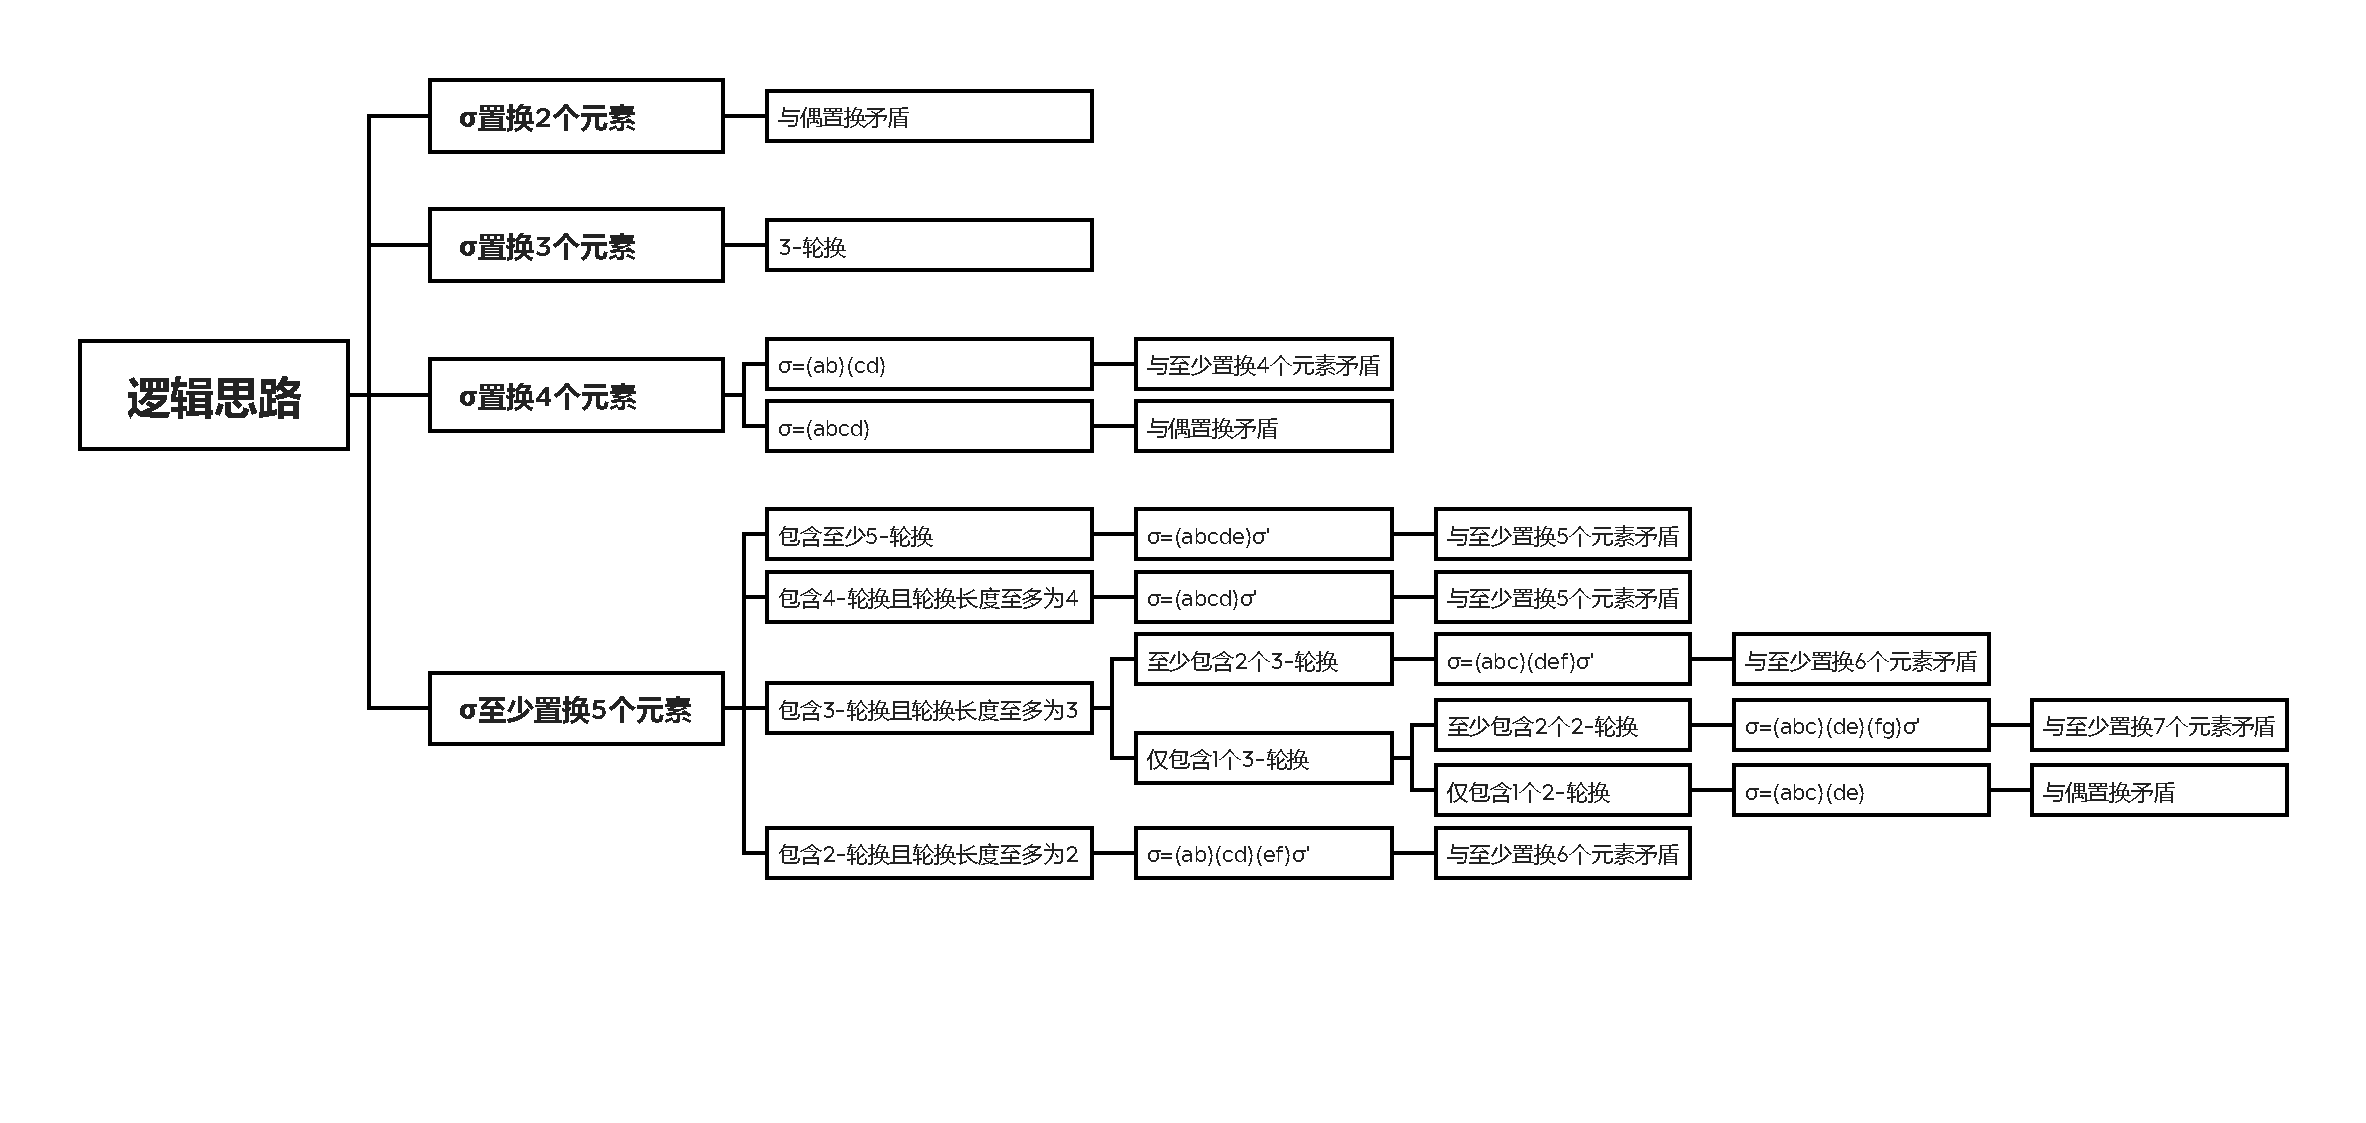
\includegraphics[scale = 0.4]{../figure/An为单群}
	\caption{逻辑思路}
\end{figure}

\begin{proof}
	在$N\lhd A_n$中取置换元素最少的非平凡置换$\sigma\in N$。
	
	如果$\sigma$置换$2$个元素,那么由引理\ref{lem:对换积的符号},这与$\sigma$为偶置换矛盾!
	
	如果$\sigma$置换$3$个元素,那么$\sigma$为$3$-轮换。
	
	如果$\sigma$置换$4$个元素,且$\sigma=(ab)(cd)$,那么由引理\ref{lem:轮换的符号},令$\tau=(cde)\in A_n$,由引理\ref{lem:轮换的共轭}
	$$
	(ab)(de)=\tau\sigma\tau^{-1}\in N\implies(cde)=\sigma\tau\sigma\tau^{-1}\in N
	$$
	这与$N$中置换至少置换$4$个元素矛盾!
	
	如果$\sigma$置换$4$个元素,且$\sigma=(abcd)$,那么由引理\ref{lem:轮换的符号},这与$\sigma$为偶置换矛盾!
	
	如果$\sigma$至少置换$5$个元素,且$\sigma$的轮换分解中包含长度至少为$5$的轮换,那么$\sigma=(abcde_1\cdots e_r)\sigma'$。由引理\ref{lem:轮换的符号},令$\tau=(bcd)\in A_n$,由引理\ref{lem:轮换的共轭}
	$$
	(acdbe_1\cdots e_r)\sigma'=\tau\sigma\tau^{-1}\in N\implies (abd)=\sigma^{-1}\tau\sigma\tau^{-1}\in N
	$$
	这与$N$中置换至少置换$5$个元素矛盾!
	
	如果$\sigma$至少置换$5$个元素,且$\sigma$的轮换分解中包含$4$-轮换,同时包含轮换长度至多为$4$,那么$\sigma=(abcd)\sigma'$。由引理\ref{lem:轮换的符号},令$\tau=(bcd)\in A_n$,由引理\ref{lem:轮换的共轭}
	$$
	(acdb)\sigma'=\tau\sigma\tau^{-1}\in N\implies (abd)=\sigma^{-1}\tau\sigma\tau^{-1}\in N
	$$
	这与$N$中置换至少置换$5$个元素矛盾!
	
	如果$\sigma$至少置换$5$个元素,且$\sigma$的轮换分解中至少包含两个$3$-轮换,同时包含轮换长度至多为$3$,那么$\sigma=(abc)(def)\sigma'$,此时$\sigma$至少置换$6$个元素。由引理\ref{lem:轮换的符号},令$\tau=(bcd)\in A_n$,由引理\ref{lem:轮换的共轭}
	$$
	(acd)(bef)\sigma'=\tau\sigma\tau^{-1}\in N\implies (abdcf)=\sigma^{-1}\tau\sigma\tau^{-1}\in N
	$$
	这与$N$中置换至少置换$6$个元素矛盾!
	
	如果$\sigma$至少置换$5$个元素,且$\sigma$的轮换分解中仅包含一个$3$-轮换,与至少两个$2$-轮换,同时包含轮换长度至多为$3$,那么$\sigma=(abc)(de)(fg)\sigma'$,此时$\sigma$至少置换$7$个元素。由引理\ref{lem:轮换的符号},令$\tau=(bcd)\in A_n$,由引理\ref{lem:轮换的共轭}
	$$
	(acd)(be)(fg)\sigma'=\tau\sigma\tau^{-1}\in N\implies (abdce)=\sigma^{-1}\tau\sigma\tau^{-1}\in N
	$$
	这与$N$中置换至少置换$7$个元素矛盾!
	
	如果$\sigma$至少置换$5$个元素,且$\sigma$的轮换分解中仅包含一个$3$-轮换,与一个$2$-轮换,那么$\sigma=(abc)(de)$,由引理\ref{lem:轮换的符号}与\ref{lem:对换积的符号}以及\ref{lem:置换复合的符号},这与$\sigma$为偶置换矛盾!
	
	如果$\sigma$至少置换$5$个元素,且$\sigma$的轮换分解中仅包含$2$-轮换,那么$\sigma=(ab)(cd)(ef)\sigma'$,此时$\sigma$至少置换$6$个元素。由引理\ref{lem:轮换的符号},令$\tau=(bcd)\in A_n$,由引理\ref{lem:轮换的共轭}
	$$
	(ac)(bd)(ef)\sigma'=\tau\sigma\tau^{-1}\in N\implies (ad)(bc)=\sigma^{-1}\tau\sigma\tau^{-1}\in N
	$$
	这与$N$中置换至少置换$6$个元素矛盾!
	
	综上所述,$\sigma$为$3$-轮换,进而命题得证!
\end{proof}

\begin{lemma}{}{3-轮换生成交错群}
	$3$-轮换生成交错群。
\end{lemma}

\begin{proof}
	由引理\ref{lem:对换生成对称群},结合
	$$
	(ab)(ac)=(acb),\qquad
	(ab)(cd)=(acb)(cda)
	$$
	命题得证!
\end{proof}

\begin{theorem}{$A_n$的单性}{An的单性}
	当且仅当$n\ne 4$时,$A_n$为单群。
\end{theorem}

\begin{proof}
	当$n\le 3$时,由命题\ref{pro:An的正规子群},$A_n$为单群。
	
	当$n=4$时,由命题\ref{pro:An的正规子群},$A_4$为非单群。
	
	当$n\ge 5$时,任取$\{\mathbbm{1}\}\subsetneq N\lhd A_n$,那么由引理\ref{lem:正规子群包含3-轮换},$N$包含$3$-轮换。由引理\ref{lem:包含1个3-轮换则包含所有3-轮换},$N$包含所有$3$-轮换。由引理\ref{lem:3-轮换生成交错群},$N=A_n$,进而$A_n$为单群。
\end{proof}

\begin{proposition}{$A_n$的交换性}{An的交换性}
	当且仅当$n\ge 4$时,$A_n$为非交换群。
\end{proposition}

\begin{proof}
	当$n=1$或$n=2$时,$A_1=\{\mathbbm{1}\}$与$A_2=\{\mathbbm{1}\}$为交换群。
	
	当$n=3$时,由命题\ref{cor:素数阶群为循环群},$A_3\cong\Z/3\Z$为交换群。
	
	当$n\ge 4$时,由引理$\ref{lem:对换积的符号}$,$(12)(13),(12)(14)\in A_4$。由于
	$$
	(12)(13)(12)(14)=(14)(23),\qquad 
	(12)(14)(12)(13)=(13)(24)
	$$
	因此$A_n$为非交换群。
\end{proof}

\begin{proposition}{$A_n$的正规子群}{An的正规子群}
	当$n\ne 4$时,$A_n$仅存在平凡正规子群。
	
	当$n=4$时,$A_4$存在且存在唯一非平凡正规子群$\Z/2\Z\times\Z/2\Z$。
\end{proposition}

\begin{proof}
	当$n=1$或$n=2$时,$A_1=\{\mathbbm{1}\}$与$A_2=\{\mathbbm{1}\}$仅存在平凡正规子群。
	
	当$n=3$时,由命题\ref{cor:素数阶群为循环群},$A_3\cong\Z/3\Z$。由命题\ref{pro:Abel单群为素数阶群},$A_3$仅存在平凡正规子群。
	
	当$n=4$时,计算可得$A_4$存在且存在唯一非平凡正规子群
	$$
	[A_4,A_4]=\{ \mathbbm{1},(12)(34),(13)(24),(14)(23) \}\cong \Z/2\Z\times\Z/2\Z
	$$
	
	当$n\ge 5$时,由定理\ref{thm:An的单性},$A_n$仅存在平凡正规子群。
\end{proof}

\begin{proposition}{$A_n$的换位子群}{An的换位子群}
	\begin{align*}
		& [A_n,A_n] = \{\mathbbm{1}\}, && n \leq 3\\
		& [A_4,A_4] \cong \Z/2\Z \times \Z/2\Z, && n = 4\\
		& [A_n,A_n] = A_n, && n \geq 5
	\end{align*}
\end{proposition}

\begin{proof}
	当$n\le 3$时,由命题\ref{pro:An的交换性}与\ref{pro:群交换的等价条件},$[A_n,A_n] = \{\mathbbm{1}\}$。
	
	当$n=4$时,由命题\ref{pro:An的正规子群},$[A_4,A_4] \cong \Z/2\Z \times \Z/2\Z$。
	
	当$n\ge 5$时,由命题\ref{pro:群的交换化}、\ref{pro:An的正规子群}、\ref{pro:An的交换性}与\ref{pro:群交换的等价条件},$[A_n,A_n] = A_n$。
\end{proof}

\begin{proposition}{$A_n$的可解性}{An的可解性}
	当且仅当$n\ge 5$时,$A_n$为不可解群。
\end{proposition}

\begin{proof}
	当$n\le 3$时,由命题\ref{pro:An的换位子群},$A_n$为可解群。
	
	当$n=4$时,由命题\ref{pro:An的换位子群}
	$$
	A_4^{(1)}\cong \Z/2\Z \times \Z/2\Z,\qquad 
	A_4^{(2)}= \{\mathbbm{1}\}
	$$
	那么$A_n$为可解群。
	
	当$n\ge 5$时,由命题\ref{pro:An的换位子群},$A_n$为不可解群。
\end{proof}

\subsection{$S_n$的结构}

\begin{table}[H]
	\centering
	\caption{$S_n$的结构}
	\begin{tabular}{|>{\centering\arraybackslash}m{1cm}|>{\centering\arraybackslash}m{1.5cm}|>{\centering\arraybackslash}m{1cm}|>{\centering\arraybackslash}m{1.5cm}|>{\centering\arraybackslash}m{3cm}|>{\centering\arraybackslash}m{2cm}|}
		\hline
		$n$     & \textbf{交换性} & \textbf{单性} & \textbf{可解性}      & \textbf{非平凡正规子群} & \textbf{换位子群}    \\
		\hline
		$1$     & $\checkmark$    & $\checkmark$ & $\checkmark$         &                       & $A_n$    \\
		\hline
		$2$     & $\checkmark$    & $\checkmark$ & $\checkmark$         &                       & $A_n$    \\
		\hline
		$3$     &                 &              & $\checkmark$         &    $A_3$              & $A_n$    \\
		\hline
		$4$     &                 &              & $\checkmark$         & $A_4,\Z/2\Z\times\Z/2\Z$  & $A_n$ \\
		\hline
		$\ge 5$ &                 & &                      &    $A_n$              & $A_n$                \\   
		\hline
	\end{tabular}
\end{table}

\begin{proposition}{$S_n$的交换性}{Sn的交换性}
	当且仅当$n\ge 3$时,$S_n$为非交换群。
\end{proposition}

\begin{proof}
	当$n=1$,$S_1=\{\mathbbm{1}\}$为交换群。
	
	当$n=2$时,由命题\ref{cor:素数阶群为循环群},$S_2\cong\Z/2\Z$为交换群。
	
	当$n\ge 3$时,由于
	$$
	(23)(132)=(12),\qquad 
	(132)(23)=(13)
	$$
	因此$S_n$为非交换群。
\end{proof}

\begin{proposition}{$S_n$的正规子群}{Sn的正规子群}
	当$n\ne 2$时,$S_n$仅存在平凡正规子群。
	
	当$n=4$时,$A_4$仅存在非平凡正规子群$A_n$与$\Z/2\Z\times\Z/2\Z$。
	
	当$n\ge 3$且$n\ne 4$时,$S_n$仅存在非平凡正规子群$A_n$。
\end{proposition}

\begin{proposition}{$S_n$的换位子群}{Sn的换位子群}
	$$
	[S_n,S_n]=A_n,\qquad n\in\N^*
	$$
\end{proposition}

\begin{proof}
	当$n\le 2$时,计算可得$[S_n,S_n]=A_n$。
	
	当$n\ge 3$时,由于
	$$
	(abc)=(bc)(ab)(bc)(ab)
	$$
	那么$3$-轮换为换位子,由引理\ref{lem:3-轮换生成交错群},$[S_n,S_n]\supset A_n$。由命题\ref{thm:交错群的指标}与命题\ref{cor:素数阶群为循环群},$S_n/A_n\cong\Z/2\Z$,因此$S_n/A_n$为交换群。由命题\ref{pro:商群交换的等价条件},$[S_n,S_n]\subset A_n$。因此$[S_n,S_n]=A_n$。
\end{proof}

\begin{proposition}{$S_n$的单性}{Sn的单性}
	当且仅当$n\ge 3$时,$S_n$为非单群。
\end{proposition}

\begin{proof}
	由命题\ref{pro:Sn的换位子群}与命题\ref{pro:群的交换化},命题得证!
\end{proof}

\begin{theorem}{$S_n$的可解性}{Sn的可解性}
	当且仅当$n\ge 5$时,$S_n$为不可解群。
\end{theorem}

\begin{proof}
	(法一)由命题\ref{pro:Sn的换位子群}与命题\ref{pro:An的可解性},命题得证!
	
	(法二)当$n\ge 5$时,由定理\ref{thm:交错群的正规性},可得次正规列
	$$
	\{\mathbbm{1}\}\lhdneq A_n \lhdneq S_n
	$$
	由定理\ref{thm:An的单性},$A_n/\{\mathbbm{1}\}=A_n$为单群。由引理\ref{thm:交错群的指标}与命题\ref{cor:素数阶群为循环群}以及命题\ref{pro:Abel单群为素数阶群},$S_n/A_n\cong \Z/2\Z$为单群。由此可知此次正规列为合成列。由命题\ref{pro:An的交换性},$A_n$不为循环群。由Jordan-Hölder定理\ref{thm:Jordan-Hölder定理}与命题\ref{pro:有限群可解的等价条件},$S_n$为不可解群。
\end{proof}

\section{群的积}

\subsection{直积}

\begin{lemma}{}{换位子群引理}
	$$
	M,N\lhd G\implies [M,N]\sub M\cap N
	$$
\end{lemma}

\begin{proof}
	这几乎是显然的,任取$m\in M$与$n\in N$,由于$M,N\lhd G$,那么
	\begin{align*}
		&n*m^{-1}*n^{-1}\in M\implies m*n*m^{-1}*n^{-1}\in M\iff [m,n]\in M\\
		&m*n*m^{-1}\in N\implies m*n*m^{-1}*n^{-1}\in N\iff [m,n]\in M
	\end{align*}
	因此$[m,n]\in M\cap N$,由$m,n$的任意性,$[M,N]\sub M\cap N$。
\end{proof}

\begin{corollary}{}{换位子群推论}
	$$
	M,N\lhd G, \quad M\cap N=\{e\}\implies \forall m\in M,\forall n\in N,m*n=n*m
	$$
\end{corollary}

\begin{proof}
	由引理\ref{lem:换位子群引理},这是显然的!
\end{proof}

\begin{proposition}{}{命题1.5.1}
	$$
	M,N\lhd G, \quad M\cap N=\{e\}\implies M\times N\cong M*N
	$$
\end{proposition}

\begin{proof}
	构造映射
	\function{\varphi}{M\times N}{M*N}{(m,n)}{m*n}
	
	首先证明$\varphi$为群同态映射,由推论\ref{cor:换位子群推论}
	\begin{align*}
		\varphi((m_1,n_1)*(m_2,n_2))
		& = \varphi((m_1*m_2,n_1*n_2))\\
		& = m_1*m_2*n_1*n_2\\
		& = m_1*n_1*m_2*n_2\\
		& = \varphi((m_1,n_1))*\varphi((m_2,n_2))
	\end{align*}
	其次证明$\varphi$为单射
	$$
	\ker\varphi=\{ (m,n)\in M\times N:m*n=e \}=\{ (m,n)\in M\times N:m,n\in M\cap N \}=\{(e,e)\}
	$$
	而显然$\varphi$为满射,因此$\varphi$为群同构映射,进而
	$$
	M\times N\cong M*N
	$$
\end{proof}

\begin{proposition}
	对于群$(G,*)$,如果$N\lhd G$且$H<G$,那么
	$$
	G=N*H,\quad N\cap H=\{e\}\iff H\cong G/N,\text{ 且群同态映射为}h\mapsto h*N
	$$
\end{proposition}

\begin{proof}
	对于必要性,如果$G=N*H$且$N\cap H=\{e\}$,那么考虑群同态映射
	\function{\varphi}{H}{G/N}{h}{h*N}
	对于单射性
	$$
	\ker\varphi=\{ h\in H:h*N=N \}=N\cap H=\{e\}
	$$
	对于满射性,任取$g\in G$,由于$G=N*H$,那么存在$n\in N$与$h\in H$,使得成立$g=n*h$,因此
	$$
	\varphi(h)=h*N=h*(h^{-1}*n*h)*N=(n*h)*N=g*N
	$$
	那么$\varphi$为群同构映射,进而$H\cong G/N$。
	
	对于充分性,如果$ H\cong G/N$,且群同态映射为
	\function{\varphi}{H}{G/N}{h}{h*N}
	由于$\varphi$为单射,那么
	$$
	M\cap N=\{ h\in H:h*N=N \}=\{ h\in H:h*N=N \}=\{e\}
	$$
	任取$g\in G$,由于$\varphi$为满射,那么存在$h\in H$,使得成立$h*N=g*N$,因此存在$n\in N$,使得成立$g=n*h$。由$g\in G$的任意性,$G=N*H$。
\end{proof}

\subsection{半直积}

\begin{definition}{半直积 semidirect product}
	定义群$(N,*)$与$(H,*)$关于群同态映射
	\function{\Psi}{H}{\mathrm{Aut}_{\mathsf{Grp}}(N)}{h}{\psi_h}
	的半直积为群$(N\rtimes_\psi H,\bullet)$,其中
	$$
	(n_1,h_1)\bullet (n_2,h_2)=(n_1*\psi_{h_1}(n_2),h_1*h_2)
	$$
\end{definition}

\begin{proposition}
	对于群$(G,*)$,如果
	$$
	N\lhd G,\quad H<G,\quad G=N*H,\quad N\cap H=\{e\}
	$$
	那么
	$$
	G\cong N\rtimes_\gamma H
	$$
	其中
	\function{\Gamma}{H}{\mathrm{Inn}_{\mathsf{Grp}}(N)}{h}{\psi_h}
\end{proposition}

\begin{proof}
	构造映射
	\function{\varphi}{N\rtimes_\psi H}{G}{(n,h)}{n*h}
	对于群同态性
	\begin{align*}
		\varphi((n_1,h_1)\bullet (n_2,h_2))
		& = \varphi((n_1*\psi_{h_1}(n_2),h_1*h_2))\\
		& = n_1*\psi_{h_1}(n_2)*h_1*h_2\\
		& = n_1*h_1*n_2*h_1^{-1}*h_1*h_2\\
		& = n_1*h_1*n_2*h_2\\
		& = \varphi((n_1,h_2))*\varphi((n_2,h_2))
	\end{align*}
	对于单射性
	$$
	\ker\varphi=\{ (n,h)\in N\rtimes_\psi H:n*h=e \}=\{ (n,h)\in N\rtimes_\psi H:n,h\in N\cap H \}=\{(e,e)\}
	$$
	而$\varphi$显然为满射,因此$\varphi$为群同构映射,进而
	$$
	G\cong N\rtimes_\gamma H
	$$
\end{proof}

\subsection{群的正合序列}

\begin{definition}{群的正合 exact of group}
	称群$G,H,K$的群同态映射序列
	$$
	\xymatrix{
	G\ar[r]^{\varphi} & H\ar[r]^{\psi} & K
	}
	$$
	在$H$处正合,如果$\im \varphi=\ker\psi$。
\end{definition}

\begin{definition}{群的正合序列 exact sequences of group}
	称群族$\{G_n\}_{n=0}^{\infty}$的群同态映射序列
	$$
	\xymatrix{
		G_0\ar[r]^{\varphi_1} & G_1\ar[r]^{\varphi_2} & G_2\ar[r]^{\varphi_3} & \cdots
	}
	$$
	为正合序列,如果对于任意$n\in\N^*$,成立$\im \varphi_n=\ker\varphi_{n+1}$。
\end{definition}

\begin{proposition}
	对于群$G$与$H$,成立
	\begin{align*}
		&\xymatrix{
			\{e\}\ar[r] & G\ar[r]^{\varphi} & H
		}\text{为群的正合序列}\iff \varphi:G\hookrightarrow H\text{为单射}\\
		&\xymatrix{
			G\ar[r]^{\varphi} & H\ar[r] & \{e\}
		}\text{为群的正合序列}\iff \varphi:G\twoheadrightarrow H\text{为满射}
	\end{align*}
\end{proposition}

\begin{proof}
	\begin{align*}
		&\xymatrix{
			\{e\}\ar[r] & G\ar[r]^{\varphi} & H
		}\text{为群的正合序列}\iff \ker\varphi=\{e\}\iff \varphi:G\hookrightarrow H\text{为单射}\\
		&\xymatrix{
			G\ar[r]^{\varphi} & H\ar[r] & \{e\}
		}\text{为群的正合序列}\iff\im\varphi=H\iff \varphi:G\twoheadrightarrow H\text{为满射}
	\end{align*}
\end{proof}

\begin{definition}{延拓 extension}
	称群$G$为群$H$关于群$N$的延拓,如果存在群的正合序列
	$$
	\xymatrix{
		\{e\} \ar[r] & N \ar[r] & G \ar[r] & H \ar[r] & \{e\}
	}
	$$
\end{definition}

\begin{definition}{分裂 split}
	称群的正合序列
	$$
	\xymatrix{
		\{e\} \ar[r] & N \ar[r] & G \ar[r] & H \ar[r] & \{e\}
	}
	$$
	为分裂的,如果存在$K<G$,使得成立$K\cong H$。
\end{definition}

\section{有限Abel群}

\subsection{有限abel群的分类}

\begin{lemma}{}{推论1.6.1}
	对于Abel群$(G,*)$,如果$H,K$为$G$的有限子群,且$\mathrm{gcd}(|H|,|K|)=1$,那么$H*K\cong H\times K$。
\end{lemma}

\begin{proof}
	由于$G$为Abel群,那么$H,K$为$G$的正规子群。由Lagrange定理\ref{thm:Lagrange定理},$H\cap K=\{e\}$。由命题\ref{pro:命题1.5.1},$H*K\cong H\times K$。
\end{proof}

\begin{corollary}{}{有限Abel群同构于其Sylow子群的积}
	有限Abel群同构于其Sylow子群的积。
\end{corollary}

\begin{proof}
	对于有限Abel群$(G,*)$,由推论\ref{cor:Sylow p-子群为正规子群的等价条件},$G$的Sylow $p$-子群唯一。记$G$的Sylow子群族为$\{ P_k \}_{k=1}^{n}$,那么对于任意$i\ne j$,成立$\mathrm{gcd}(|P_i|,|P_j|)=1$,因此由引理\ref{lem:推论1.6.1}
	$$
	G=P_1*\cdots *P_n\cong P_1\times\cdots\times P_n
	$$
\end{proof}

\begin{lemma}
	对于素数$p$与$r\in\N^*$,如果$(G,*)$为$p^{r+1}$阶非循环Abel群,且$g\in G$为$p^r$阶元素,那么存在$p$阶元素$h\in G\setminus\lang g\rang$。
\end{lemma}

\begin{proof}
	由于$G$为Abel群,那么$\langle g \rangle \lhd G$,因此商群$G/\lang g\rang$的阶为$p$。任取$k\in G\setminus\lang g\rang$,由Lagrange定理\ref{thm:Lagrange定理},$p\mid|k|$,且$k*\langle g \rangle$的阶为$p$,因此$k^p\in \langle g \rangle$。由Lagrange定理\ref{thm:Lagrange定理},$k^p$的阶为$p$的幂。
	
	令$|k^p|=p^s$,其中$0\le s \le r$。由命题\ref{pro:元素的幂的阶},$|k|=p|k^p|=p^{s+1}$。如果$s=r$,那么$|k|=p^{r+1}$,因此$G\cong \langle k \rangle$,与$G$为非循环群矛盾!进而$s< r$。由命题\ref{pro:有限循环群的子群结构},$\langle k^p \rangle\=\langle g^{p^{r-s}} \rangle\sub \langle g^p \rangle$,因此存在$n\in\Z$,使得成立$k^p=g^{np}$。令$h=k*g^{-n}\in G\setminus\lang g\rang$,那么$h\ne e$,且$h^p=e$,于是$|h|=p$。
\end{proof}

\begin{lemma}{}{引理163}
	对于Abel $p$-群$(G,*)$,如果$g\in G$为其阶最大的元素,那么存在$H<G$,使得成立$G=H*\lang g\rang$,且$H\cap \lang g\rang=\{e\}$。
\end{lemma}

\begin{corollary}{Abel $p$-群的结构}{Abelp群的结构}
	Abel $p$-群同构于循环$p$-群的积。
\end{corollary}

\begin{proof}
	对于Abel $p$-群$(G,*)$,对于$|G|$进行数学归纳证明。如果$|G|=1$,那么$G\cong \{e\}$。
	
	如果$|G|<n$时命题成立,那么当$|G|=n$时,取$G$中阶最大的元素$g$,由引理\ref{lem:引理163},存在$H<G$,使得成立$G=H*\lang g\rang$。由归纳假设,$H$同构于循环$p$-群的积,那么$G$同构于循环$p$-群的积。
	
	由数学归纳法,命题得证!
\end{proof}

\begin{corollary}{}{有限Abel群的结构}
	有限Abel群可表示为循环$p$-群的积。
\end{corollary}

\begin{proof}
	对于有限Abel群$(G,*)$,由推论\ref{cor:有限Abel群同构于其Sylow子群的积}
	$$
	G=P_1*\cdots *P_n\cong P_1\times\cdots\times P_n
	$$
	其中$\{ P_k \}_{k=1}^{n}$为$G$的Sylow子群族。由推论\ref{cor:Abelp群的结构},每一个$P_k$同构于循环$p$-群的积,其中$1\le k\le n$,那么$G$同构于循环$p$-群的积。
\end{proof}

\subsection{有限Abel群的结构定理}

\begin{theorem}{有限Abel群的结构定理}{有限Abel群的结构定理}
	\begin{enumerate}
		\item 对于互异素数$p_1,\cdots,p_n$,$p_1^{r_1}\cdots p_n^{r_n}$阶Abel群的结构为
		$$
		\bigotimes_{i=1}^{n}\bigotimes_{j=1}^{k_i}\frac{\Z}{p_i^{r_i^{(j)}}\Z}
		$$
		其中对于任意$1\le i\le n$,成立
		$$
		r_i^{(1)}\le\cdots \le r_i^{(k_i)},\qquad 
		r_i^{(1)}+\cdots+r_i^{(k_i)}=r_i
		$$
		\item 有限Abel群的结构为
		$$
		\frac{\Z}{d_1\Z}\times\cdots\times\frac{\Z}{d_n\Z}
		$$
		其中$1<d_1\mid \cdots \mid d_n$。
	\end{enumerate}
\end{theorem}

\subsection{域的乘法群的有限子群}

\begin{lemma}{}{有限Abel群为循环群的充分条件}
	对于有限Abel群$(G,*)$,如果对于任意$n\in\N^*$,成立$|G_n|\le n$,其中
	$$
	G_n=\{ g\in G:g^n=e \}
	$$
	为$G$的子群,那么$G$为循环群。
\end{lemma}

\begin{proof}
	由有限Abel群的结构定理\ref{thm:有限Abel群的结构定理},存在$1<d_1\mid \cdots \mid d_m$,使得成立
	$$
	G\cong \frac{\Z}{d_1\Z}\times\cdots\times\frac{\Z}{d_n\Z}
	$$
	如果$m\ge 2$,那么
	$$
	|G|=d_1\cdots d_m>d_m
	$$
	但是对于任意$g\in G$,成立$g^{d_m}=e$,因此$G_{d_m}=G$,于是
	$$
	|G_{d_m}|=|G|>d_m
	$$
	与假设矛盾!进而$m=1$,那么$G\cong \Z/d_1\Z$为循环群。
\end{proof}

\begin{theorem}{域的乘法群的有限子群为循环群}{域的乘法群的有限子群为循环群}
	对于域$(F,+,\;\cdot\;)$,如果$G$为乘法群$(F^{\times},\;\cdot\;)$的有限子群,那么$G$为循环群。
\end{theorem}

\begin{proof}
	考察$G$的子群
	$$
	G_n=\{ g\in G:g^n=1 \}
	$$
	考虑域$F$上的$n$次多项式$f(x)=x^n-1$,那么$G_n$中的元素均为$f(x)$在$F$中的根。由引理\ref{lem:n次多项式至多存在n个根},$f(x)$在$F$中至多存在$n$个根,则$|G_n|\le n$,进而由引理\ref{lem:有限Abel群为循环群的充分条件},$G$为循环群。
\end{proof}

% \end{document}
